%% Beginning of file 'sample631.tex'
%%
%% Modified 2021 March
%%
%% This is a sample manuscript marked up using the
%% AASTeX v6.31 LaTeX 2e macros.
%%
%% AASTeX is now based on Alexey Vikhlinin's emulateapj.cls 
%% (Copyright 2000-2015).  See the classfile for details.

%% AASTeX requires revtex4-1.cls and other external packages such as
%% latexsym, graphicx, amssymb, longtable, and epsf.  Note that as of 
%% Oct 2020, APS now uses revtex4.2e for its journals but remember that 
%% AASTeX v6+ still uses v4.1. All of these external packages should 
%% already be present in the modern TeX distributions but not always.
%% For example, revtex4.1 seems to be missing in the linux version of
%% TexLive 2020. One should be able to get all packages from www.ctan.org.
%% In particular, revtex v4.1 can be found at 
%% https://www.ctan.org/pkg/revtex4-1.

%% The first piece of markup in an AASTeX v6.x document is the \documentclass
%% command. LaTeX will ignore any data that comes before this command. The 
%% documentclass can take an optional argument to modify the output style.
%% The command below calls the preprint style which will produce a tightly 
%% typeset, one-column, single-spaced document.  It is the default and thus
%% does not need to be explicitly stated.
%%
%% using aastex version 6.3

\documentclass[]{aastex631}
%% The default is a single spaced, 10 point font, single spaced article.
%% There are 5 other style options available via an optional argument. They
%% can be invoked like this:
%%
%% \documentclass[arguments]{aastex631}
%% 
%% where the layout options are:
%%
%%  twocolumn   : two text columns, 10 point font, single spaced article.
%%                This is the most compact and represent the final published
%%                derived PDF copy of the accepted manuscript from the publisher
%%  manuscript  : one text column, 12 point font, double spaced article.
%%  preprint    : one text column, 12 point font, single spaced article.  
%%  preprint2   : two text columns, 12 point font, single spaced article.
%%  modern      : a stylish, single text column, 12 point font, article with
%% 		  wider left and right margins. This uses the Daniel
%% 		  Foreman-Mackey and David Hogg design.
%%  RNAAS       : Supresses an abstract. Originally for RNAAS manuscripts 
%%                but now that abstracts are required this is obsolete for
%%                AAS Journals. Authors might need it for other reasons. DO NOT
%%                use \begin{abstract} and \end{abstract} with this style.
%%
%% Note that you can submit to the AAS Journals in any of these 6 styles.
%%
%% There are other optional arguments one can invoke to allow other stylistic
%% actions. The available options are:
%%
%%   astrosymb    : Loads Astrosymb font and define \astrocommands. 
%%   tighten      : Makes baselineskip slightly smaller, only works with 
%%                  the twocolumn substyle.
%%   times        : uses times font instead of the default
%%   linenumbers  : turn on lineno package.
%%   trackchanges : required to see the revision mark up and print its output
%%   longauthor   : Do not use the more compressed footnote style (default) for 
%%                  the author/collaboration/affiliations. Instead print all
%%                  affiliation information after each name. Creates a much 
%%                  longer author list but may be desirable for short 
%%                  author papers.
%% twocolappendix : make 2 column appendix.
%%   anonymous    : Do not show the authors, affiliations and acknowledgments 
%%                  for dual anonymous review.
%%
%% these can be used in any combination, e.g.
%%
%% \documentclass[twocolumn,linenumbers,trackchanges]{aastex631}
%%
%% AASTeX v6.* now includes \hyperref support. While we have built in specific
%% defaults into the classfile you can manually override them with the
%% \hypersetup command. For example,
%%
%% \hypersetup{linkcolor=red,citecolor=green,filecolor=cyan,urlcolor=magenta}
%%
%% will change the color of the internal links to red, the links to the
%% bibliography to green, the file links to cyan, and the external links to
%% magenta. Additional information on \hyperref options can be found here:
%% https://www.tug.org/applications/hyperref/manual.html#x1-40003
%%
%% Note that in v6.3 "bookmarks" has been changed to "true" in hyperref
%% to improve the accessibility of the compiled pdf file.
%%
%% If you want to create your own macros, you can do so
%% using \newcommand. Your macros should appear before
%% the \begin{document} command.
%%

\DeclareUnicodeCharacter{2212}{-} 


%\usepackage{amsmath}	% Advanced maths commands


%\usepackage{placeins}
\usepackage[figuresleft]{rotating}
\usepackage{xspace}

\newcommand{\vdag}{(v)^\dagger}
\newcommand\aastex{AAS\TeX}
\newcommand\latex{La\TeX}

\newcommand{\g}{GALAH\xspace}
\newcommand{\ts}{t-SNE\xspace}
\newcommand{\mps}{metal-poor}
\newcommand{\emp}{EMP star\xspace}
\newcommand{\emps}{EMP stars\xspace}
\newcommand{\logg}{\ensuremath{\log g}\xspace}
\newcommand{\teff}{\ensuremath{T_{\mathrm{eff}}}\xspace}  
\newcommand{\Ha}{H$\alpha$}
\newcommand{\Hb}{H$\beta$}
\newcommand{\feh}{[Fe/H]\xspace}
\newcommand{\ci}{$\chi^2$\xspace}
\renewcommand{\tabcolsep}{1.5pt}


\usepackage{amssymb}	% Extra maths symbols
\usepackage{nicefrac}
\usepackage{comment}
\usepackage{subfig}
\usepackage{gensymb}
\usepackage{enumitem}

%% Reintroduced the \received and \accepted commands from AASTeX v5.2
%\received{March 1, 2021}
%\revised{April 1, 2021}
%\accepted{\today}

%% Command to document which AAS Journal the manuscript was submitted to.
%% Adds "Submitted to " the argument.
%\submitjournal{PSJ}

%% For manuscript that include authors in collaborations, AASTeX v6.31
%% builds on the \collaboration command to allow greater freedom to 
%% keep the traditional author+affiliation information but only show
%% subsets. The \collaboration command now must appear AFTER the group
%% of authors in the collaboration and it takes TWO arguments. The last
%% is still the collaboration identifier. The text given in this
%% argument is what will be shown in the manuscript. The first argument
%% is the number of author above the \collaboration command to show with
%% the collaboration text. If there are authors that are not part of any
%% collaboration the \nocollaboration command is used. This command takes
%% one argument which is also the number of authors above to show. A
%% dashed line is shown to indicate no collaboration. This example manuscript
%% shows how these commands work to display specific set of authors 
%% on the front page.
%%
%% For manuscript without any need to use \collaboration the 
%% \AuthorCollaborationLimit command from v6.2 can still be used to 
%% show a subset of authors.
%
%\AuthorCollaborationLimit=2
%
%% will only show Schwarz & Muench on the front page of the manuscript
%% (assuming the \collaboration and \nocollaboration commands are
%% commented out).
%%
%% Note that all of the author will be shown in the published article.
%% This feature is meant to be used prior to acceptance to make the
%% front end of a long author article more manageable. Please do not use
%% this functionality for manuscripts with less than 20 authors. Conversely,
%% please do use this when the number of authors exceeds 40.
%%
%% Use \allauthors at the manuscript end to show the full author list.
%% This command should only be used with \AuthorCollaborationLimit is used.

%% The following command can be used to set the latex table counters.  It
%% is needed in this document because it uses a mix of latex tabular and
%% AASTeX deluxetables.  In general it should not be needed.
%\setcounter{table}{1}

%%%%%%%%%%%%%%%%%%%%%%%%%%%%%%%%%%%%%%%%%%%%%%%%%%%%%%%%%%%%%%%%%%%%%%%%%%%%%%%%
%%
%% The following section outlines numerous optional output that
%% can be displayed in the front matter or as running meta-data.
%%
%% If you wish, you may supply running head information, although
%% this information may be modified by the editorial offices.
\shorttitle{Extremely Metal-Poor Stars in GALAH}
\shortauthors{Hughes et al.}
%%
%% You can add a light gray and diagonal water-mark to the first page 
%% with this command:
%% \watermark{text}
%% where "text", e.g. DRAFT, is the text to appear.  If the text is 
%% long you can control the water-mark size with:
%% \setwatermarkfontsize{dimension}
%% where dimension is any recognized LaTeX dimension, e.g. pt, in, etc.
%%
%%%%%%%%%%%%%%%%%%%%%%%%%%%%%%%%%%%%%%%%%%%%%%%%%%%%%%%%%%%%%%%%%%%%%%%%%%%%%%%%
\graphicspath{{./}{figures/}}
%% This is the end of the preamble.  Indicate the beginning of the
%% manuscript itself with \begin{document}.

\begin{document}

\title{The GALAH Survey: A New Sample of Extremely Metal-Poor Stars Using A Machine Learning Classification Algorithm}

%% LaTeX will automatically break titles if they run longer than
%% one line. However, you may use \\ to force a line break if
%% you desire. In v6.31 you can include a footnote in the title.

%% A significant change from earlier AASTEX versions is in the structure for 
%% calling author and affiliations. The change was necessary to implement 
%% auto-indexing of affiliations which prior was a manual process that could 
%% easily be tedious in large author manuscripts.
%%
%% The \author command is the same as before except it now takes an optional
%% argument which is the 16 digit ORCID. The syntax is:
%% \author[xxxx-xxxx-xxxx-xxxx]{Author Name}
%%
%% This will hyperlink the author name to the author's ORCID page. Note that
%% during compilation, LaTeX will do some limited checking of the format of
%% the ID to make sure it is valid. If the "orcid-ID.png" image file is 
%% present or in the LaTeX pathway, the OrcID icon will appear next to
%% the authors name.
%%
%% Use \affiliation for affiliation information. The old \affil is now aliased
%% to \affiliation. AASTeX v6.31 will automatically index these in the header.
%% When a duplicate is found its index will be the same as its previous entry.
%%
%% Note that \altaffilmark and \altaffiltext have been removed and thus 
%% can not be used to document secondary affiliations. If they are used latex
%% will issue a specific error message and quit. Please use multiple 
%% \affiliation calls for to document more than one affiliation.
%%
%% The new \altaffiliation can be used to indicate some secondary information
%% such as fellowships. This command produces a non-numeric footnote that is
%% set away from the numeric \affiliation footnotes.  NOTE that if an
%% \altaffiliation command is used it must come BEFORE the \affiliation call,
%% right after the \author command, in order to place the footnotes in
%% the proper location.
%%
%% Use \email to set provide email addresses. Each \email will appear on its
%% own line so you can put multiple email address in one \email call. A new
%% \correspondingauthor command is available in V6.31 to identify the
%% corresponding author of the manuscript. It is the author's responsibility
%% to make sure this name is also in the author list.
%%
%% While authors can be grouped inside the same \author and \affiliation
%% commands it is better to have a single author for each. This allows for
%% one to exploit all the new benefits and should make book-keeping easier.
%%
%% If done correctly the peer review system will be able to
%% automatically put the author and affiliation information from the manuscript
%% and save the corresponding author the trouble of entering it by hand.

%\correspondingauthor{August Muench}
%\email{greg.schwarz@aas.org, gus.muench@aas.org}

\author[0000-0001-9294-3089]{Arvind C.N. Hughes} %Corrected ORCID number
\affiliation{School of Mathematical and Physical Sciences, Macquarie University, Sydney, NSW 2109, Australia}
\affiliation{Research Centre in Astronomy, Astrophysics \& Astrophotonics, Macquarie University, Sydney, NSW 2109, Australia}
\affiliation{Centre of Excellence for Astrophysics in Three Dimensions (ASTRO-3D), Australia}
\affiliation{Max Planck Institute for Astronomy, Heidelberg, Germany}

\author[0000-0001-5185-9876]{Lee R. Spitler}
\affiliation{School of Mathematical and Physical Sciences, Macquarie University, Sydney, NSW 2109, Australia}
\affiliation{Research Centre in Astronomy, Astrophysics \& Astrophotonics, Macquarie University, Sydney, NSW 2109, Australia}
\affiliation{Centre of Excellence for Astrophysics in Three Dimensions (ASTRO-3D), Australia}
\affiliation{Australian Astronomical Optics, Faculty of Science and Engineering, Macquarie University, Macquarie Park, NSW 2113, Australia}



\author[0000-0003-1124-8477]{Daniel B. Zucker}
\affiliation{School of Mathematical and Physical Sciences, Macquarie University, Sydney, NSW 2109, Australia}
\affiliation{Research Centre in Astronomy, Astrophysics \& Astrophotonics, Macquarie University, Sydney, NSW 2109, Australia}
\affiliation{Centre of Excellence for Astrophysics in Three Dimensions (ASTRO-3D), Australia}

\author[0000-0001-5344-8069]{Thomas Nordlander}
\affiliation{Research School of Astronomy and Astrophysics, Australian National University, ACT 2611, Australia}
\affiliation{ARC Centre of Excellence for All Sky Astrophysics in 3 Dimensions (ASTRO 3D)}

\author[0000-0002-8165-2507]{Jeffrey Simpson}
\affiliation{School of Physics, UNSW, Sydney, NSW 2052, Australia}
\affiliation{ARC Centre of Excellence for All Sky Astrophysics in 3 Dimensions (ASTRO 3D)}

\author[0000-0001-7019-649X]{Gary S. Da Costa}
\affiliation{Research School of Astronomy and Astrophysics, Australian National University, ACT 2611, Australia}
\affiliation{ARC Centre of Excellence for All Sky Astrophysics in 3 Dimensions (ASTRO 3D)}

\author[0000-0001-5082-9536]{Yuan-Sen Ting}
\affiliation{Research School of Astronomy and Astrophysics, Australian National University, ACT 2611, Australia}
\affiliation{Research School of Computer Science, Australian National University, Acton ACT 2601, Australia}



\author[0000-0002-3084-5157]{Chengyuan Li}
\affiliation{School of Physics and Astronomy, Sun Yat-sen University, Zhuhai, Guangdong, China}

\author[0000-0001-7516-4016]{Joss~Bland-Hawthorn}
\affiliation{Sydney Institute for Astronomy, School of Physics, A28, The University of Sydney, NSW 2006, Australia}
\affiliation{Centre of Excellence for Astrophysics in Three Dimensions (ASTRO-3D), Australia}

\author[0000-0002-4031-8553]{Sven~Buder}
\affiliation{Research School of Astronomy and Astrophysics, Australian National University, ACT 2611, Australia}
\affiliation{Centre of Excellence for Astrophysics in Three Dimensions (ASTRO-3D), Australia}

\author[0000-0003-0174-0564]{Andrew~R.~Casey}
\affiliation{Monash Centre for Astrophysics, Monash University, Australia}
\affiliation{School of Physics and Astronomy, Monash University, Australia}

\author[0000-0001-7362-1682]{Gayandhi~M.~De~Silva}
\affiliation{Australian Astronomical Optics, Faculty of Science and Engineering, Macquarie University, Macquarie Park, NSW 2113, Australia}
\affiliation{Research Centre in Astronomy, Astrophysics \& Astrophotonics, Macquarie University, Sydney, NSW 2109, Australia}


\author[0000-0002-2662-3762]{Valentina~{D'Orazi}}
\affiliation{Istituto Nazionale di Astrofisica, Osservatorio Astronomico di Padova, vicolo dell'Osservatorio 5, 35122, Padova, Italy}

\author[0000-0001-6280-1207]{Ken~C.~Freeman}
\affiliation{Research School of Astronomy and Astrophysics, Australian National University, ACT 2611, Australia}

\author[0000-0001-7294-9766]{Michael~R.~Hayden}
\affiliation{Sydney Institute for Astronomy, School of Physics, A28, The University of Sydney, NSW 2006, Australia}
\affiliation{Centre of Excellence for Astrophysics in Three Dimensions (ASTRO-3D), Australia}

\author{Janez~Kos}
\affiliation{Faculty of Mathematics and Physics, University of Ljubljana, Jadranska 19, 1000 Ljubljana, Slovenia}

\author[0000-0003-3081-9319]{Geraint~F.~Lewis}
\affiliation{Sydney Institute for Astronomy, School of Physics, A28, The University of Sydney, NSW 2006, Australia}

\author{Jane~Lin}
\affiliation{Research School of Astronomy and Astrophysics, Australian National University, ACT 2611, Australia}
\affiliation{Centre of Excellence for Astrophysics in Three Dimensions (ASTRO-3D), Australia}

\author{Karin~Lind}
\affiliation{Department of Astronomy, Stockholm University, AlbaNova University Centre, SE-106 91 Stockholm, Sweden}

\author[0000-0002-3430-4163]{Sarah~L.~Martell}
\affiliation{School of Physics, UNSW, Sydney, NSW 2052, Australia}
\affiliation{Centre of Excellence for Astrophysics in Three Dimensions (ASTRO-3D), Australia}

\author[0000-0003-0110-0540]{Katharine J. Schlesinger}
\affiliation{Research School of Astronomy and Astrophysics, Australian National University, ACT 2611, Australia}

\author[0000-0002-0920-809X]{Sanjib~Sharma}
\affiliation{Sydney Institute for Astronomy, School of Physics, A28, The University of Sydney, NSW 2006, Australia}
\affiliation{Centre of Excellence for Astrophysics in Three Dimensions (ASTRO-3D), Australia}

\author[0000-0002-2325-8763]{Toma\v{z}~Zwitter}
\affiliation{Faculty of Mathematics and Physics, University of Ljubljana, Jadranska 19, 1000 Ljubljana, Slovenia}

\author{the GALAH Collaboration}

%% Note that the \and command from previous versions of AASTeX is now
%% depreciated in this version as it is no longer necessary. AASTeX 
%% automatically takes care of all commas and "and"s between authors names.

%% AASTeX 6.31 has the new \collaboration and \nocollaboration commands to
%% provide the collaboration status of a group of authors. These commands 
%% can be used either before or after the list of corresponding authors. The
%% argument for \collaboration is the collaboration identifier. Authors are
%% encouraged to surround collaboration identifiers with ()s. The 
%% \nocollaboration command takes no argument and exists to indicate that
%% the nearby authors are not part of surrounding collaborations.

%% Mark off the abstract in the ``abstract'' environment. 
\begin{abstract}


Extremely Metal-Poor (EMP) stars provide a valuable probe of early chemical enrichment in the Milky Way. Here we leverage a large sample of $\sim600,000$ high-resolution stellar spectra from the GALAH survey plus a machine learning algorithm to find 54 candidates with estimated [Fe/H]~$\leq$~-3.0, 6 of which have [Fe/H]~$\leq$~-3.5. Our sample includes $\sim 20 \%$ main sequence EMP candidates, unusually high for \emp surveys. We find the magnitude-limited metallicity distribution function of our sample is consistent with previous work that used more complex selection criteria.  The method we present has significant potential for application to the next generation of massive stellar spectroscopic surveys, which will expand the available spectroscopic data well into the millions of stars. 

\end{abstract}

%% Keywords should appear after the \end{abstract} command. 
%% The AAS Journals now uses Unified Astronomy Thesaurus concepts:
%% https://astrothesaurus.org
%% You will be asked to selected these concepts during the submission process
%% but this old "keyword" functionality is maintained in case authors want
%% to include these concepts in their preprints.
\keywords{Stellar classification (1589), Astronomy data analysis (1858)}

%% From the front matter, we move on to the body of the paper.
%% Sections are demarcated by \section and \subsection, respectively.
%% Observe the use of the LaTeX \label
%% command after the \subsection to give a symbolic KEY to the
%% subsection for cross-referencing in a \ref command.
%% You can use LaTeX's \ref and \label commands to keep track of
%% cross-references to sections, equations, tables, and figures.
%% That way, if you change the order of any elements, LaTeX will
%% automatically renumber them.
%%
%% We recommend that authors also use the natbib \citep
%% and \citet commands to identify citations.  The citations are
%% tied to the reference list via symbolic KEYs. The KEY corresponds
%% to the KEY in the \bibitem in the reference list below. 

\section{Introduction} \label{sec:intro}

Extremely metal-poor stars (EMP, [Fe/H] $\leq$ –3.0) are interesting stellar objects, as they provide a window into the history of the early Universe. The \emps \ that exist today formed in environments with much less chemical enrichment than is typically found in the interstellar medium today. As a result, they record the chemical yields produced by the first generations of stars after the Big Bang, and thereby provide crucial clues to the properties of early supernovae and their progenitors.  Hence \emps \ are essentially a log of some of the earliest events in the Galaxy's chemical evolution.

 The significance of metal-poor stars has been be reviewed extensively \citep[e.g.,][]{Beers2005,Frebel2015}. However, to date very few EMP stars have been discovered, especially considering the fact that entire observational surveys have been dedicated to that aim.
Querying the high-resolution SAGA database \citep{2008PASJ...60.1159S} we see only $\sim{1000} ~\mathrm{stars}~\mathrm{with ~\feh} < -3$, $\sim{200} ~\mathrm{with ~\feh} < -3.5$ and $\sim{50} ~\mathrm{with ~\feh} < -4$ have been found. 
As noted above, \emps offer a unique window into the chemical enrichment of the Milky Way as it was forming, yet their relative rarity constrains our ability to probe those early times. Hence expanding the known sample is of critical importance for creating a comprehensive picture of the processes dominating the life cycle of stars and the interstellar medium in the early Universe.


With the development of highly multiplexed astronomical spectrographs, many current stellar surveys are producing spectroscopic datasets that are too large for traditional analysis (e.g., RAVE \citealt{Steinmetz_2020}; APOGEE \citealt{SDSS-IV:2019};  GALAH \citealt{buder_2020}). The next generation of surveys -- including WEAVE \citep{Dalton_2014}, 4MOST \citep{Jong20194MOSTPO} and SDSS V's MWM \citep{kollmeier2017sdssv} -- will expand the available spectroscopic data well into the millions of stars.
Thanks to recent improvements in computing and statistical methods however, we are now able to develop more refined tools and processes to sift through these huge datasets in order to reliably identify rare and interesting science targets, such as \emps. This paper seeks to identify \emps in the GALAH spectroscopic survey, and develops a novel machine-learning approach that could be used to identify other scarce objects in large astronomical datasets.


 The machine learning method adopted in this paper is \ts \citep{maaten_visualizing_2008}, a dimensionality reduction technique. This method has been successfully applied to astronomical data for identification of sub-structure within a parameter space and the classification of stellar objects; in particular, \ts has been applied in the stellar and chemical abundance space, to identify membership in stellar-clusters and streams \citep[e.g.,][]{2018A&A...619A.125A,2018MNRAS.473.4612K}. \cite{2017A&A...603A..19M} and \cite{2017MNRAS.472.2517J} applied \ts to RAVE survey spectra to identify very metal-poor stars and stellar twins, respectively, and \cite{2020A&A...638A.145T} used \ts on GALAH spectra to find FGK-type binary stars. The application of \ts in these cases followed a top-down approach, i.e., running \ts on the dataset in question and then exploring the resulting space, which can be inefficient in identifying objects of particular interest. In this paper however, we show an alternative approach, following the process described in \cite{hughes2017} and similar to \cite{hawkins2021}, in which we flag objects we are interested in prior to running \ts, and then see where they appear on the projected \ts space. This works because any unclassified star falling near the flagged stars can be considered a potential candidate because it will have similar spectral features.

In this paper, data from the GALactic Archaeology with HERMES spectroscopic survey (GALAH) are analysed to show how machine learning methods, applied to spectra, can be used to identify extremely metal-poor stars. The paper is organised as follows: the GALAH survey and the data are described in Section~\ref{Sec:Data}, Section~\ref{Sec:Method} outlines the methodology used to find \emps, the results and candidates from applying the methodology to the data are shown in Section~\ref{Sec:Results}, in Section~\ref{Sec:Discussion} we discuss those results and we summarise our conclusions in Section~\ref{Sec:Conclusions}.


\begin{table}
\centering
\scalebox{0.8}{
\hskip-4.0cm\begin{tabular}{lllrr|rrr|lrr@{}}  
\hline
  \tt s\_object\_ID &
   \tt Object Name &               
  \tt $\mathrm{T^{L}_{eff}}$ &
  \tt $\mathrm{log \ g^{L}}$ &
 \tt $\mathrm{[Fe/H]^{L}}$ &
  $\mathrm{T^{Est}_{eff}}$ &
  $\mathrm{log \ g^{Est}}$ &
  $\mathrm{[Fe/H]^{Est}}$ &
  \tt $\mathrm{T^{DR3}_{eff}}$ &
  \tt $\mathrm{log \ g^{DR3}}$ &
  \tt $\mathrm{[Fe/H]^{DR3}}$ 
   \\
   \hline
   \hline
140209005201151* & HD 122563 ~\cite{2010ApJS..191..352K}   & 4367 & 0.60 & -3.15 & 5000 & 0.50 & -2.80 & 4616 & 1.46 & -2.51 \\
140307003101095 & 2MASS   J13274506-4732201 ~\cite{2012MNRAS.427.1153S}  & 4661 & 1.50 & -2.70 & 5000 & 0.50 & -2.10 & 4616 & 1.36 & -1.87 \\
140412001201388 & HE 1207-3108 ~\cite{Yong_2012}  & 5294 & 2.85 & -2.70 & 5300 & 0.50 & -3.10 & 5404 & 2.97 & -2.56 \\
140810004701232 & UCAC4 157-208544 ~\cite{2019ApJ...870..122P}  & 4651 & 1.24 & -2.52 & 5000 & 0.50 & -2.10 & 4539 & 1.46 & -1.87 \\
150409002601337 & TYC 4934-700-1~\cite{2018ApJ...868..110S}  & 4614 & 1.03 & -2.52 & 5100 & 0.50 & -2.60 & 4687 & 1.45 & -2.25 \\
150718004401358* & BPS CS 22892-0052 ~\cite{1995AJ....109.2757M} & 4760 & 1.30 & -3.10 & 5200 & 3.75 & -3.50 & 5657 & 2.33 & -2.19 \\
151008003501121* & HE 0124-0119 ~\cite{Li_2015} & 4330 & 0.10 & -3.57 & 4000 & 5.00 & -4.25 & 4367 & 1.63 & -3.38 \\
160401003901201 & DENIS J133748.8-082617~\cite{2018ApJ...868..110S}  & 4265 & 0.25 & -2.62 & 4800 & 0.50 & -2.40 & 4289 & 0.73 & -2.44 \\
160403004201044 & 2MASS J13273676-1710384 ~\cite{2019ApJ...870..122P}  & 5223 & 1.67 & -2.55 & 5200 & 0.75 & -2.60 & 5127 & 2.12 & -2.17 \\
160424004701042 & UCAC4 053-017641~\cite{2019ApJ...870..122P}  & 4832 & 1.61 & -3.41 & 5000 & 0.50 & -2.90 & 4795 & 2.05 & -2.51 \\
160519002601142 & UCAC4 226-057537~\cite{2019ApJ...870..122P} & 4619 & 1.07 & -2.54 & 4900 & 0.50 & -2.30 & 4526 & 1.40 & -2.05 \\
160813003601164* & 2MASS J21260896-0316587 ~\cite{2011ApJ...742...54H}& 4725 & 1.15 & -3.22 & 5100 & 0.50 & -3.10 & 5056 & 2.15 & -2.71 \\
161009003801062 & UCAC4 464-129364~\cite{Mardini_2019}& 4945 & 1.53 & -2.52 & 5000 & 0.50 & -2.70 & 4743 & 2.10 & -2.36 \\
161104002301201 & 2MASS J22045836+0401321~\cite{2018AA...611A..30S} & 4700 & 1.20 & -2.90 & 5000 & 0.50 & -2.80 & 4632 & 1.82 & -2.57 \\
161118004701028 & SMSS J051008.62-372019.8 ~\cite{2015ApJ...807..171J} & 5170 & 2.40 & -3.20 & 5300 & 0.50 & -3.20 & 5342 & 3.31 & -2.68 \\
170601003101219 & 2MASS J14175995-2415463~\cite{Schlaufman_2014}  & 4914 & 1.45 & -2.40 & 5000 & 0.50 & -2.60 & 4724 & 1.47 & -2.21 \\
170615004401258* & 2MASS J18082002-5104378~\cite{mele} & 5440 & 3.00 & -4.07 & 5500 & 0.50 & -4.25 & 5741 & 3.48 &  \nodata \\
170805005101110 & HE 0048-6408~\cite{2014ApJ...781...40P} & 4378 & 0.15 & -3.75 & 4800 & 0.50 & -3.80 & 4221 & 1.18 & -3.83 \\
170904000601186 & 2MASS J21303218-4616247~\cite{2010AA...509A..93M} & 4100 & -0.30 & -3.39 & 5000 & 0.50 & -3.10 & 3987 & 0.89 & -3.76 \\
170906004601038 & HE 0105-6141 ~\cite{2005AA...439..129B} & 5218 & 2.83 & -2.55 & 5300 & 0.75 & -2.60 & 5190 & 2.87 & -2.36 \\
170906004601108 & BPS CS 22953-0003~\cite{2018AA...611A..30S} & 5100 & 2.30 & -2.80 & 5100 & 0.50 & -3.10 & 5044 & 2.36 & -2.73 \\
171001003401116 & HE 0433-1008~\cite{2017ApJ...835...81B}  & 4708 & 1.31 & -2.62 & 4900 & 0.50 & -2.70 & 4423 & 1.54 & -2.77 \\
171205002101255* & SMSS J031300.36-670839.3~[{Keller}]\cite{Nordlander2017} & 5150 & 2.20 & $~<-6.53$ & 5000 & \nodata & \nodata & \nodata & \nodata & \nodata \\ 
\hline

\end{tabular}
}
\caption{Extremely metal-poor stars from the literature found in GALAH DR3, designated with the GALAH identifier {\tt  s\_object\_ID}. The different superscripts in the stellar parameters reflect the source of the parameters: {\bf L} indicates values from the literature, {\bf Est} shows the results of our parameter estimation method and {\bf DR3} represents the output of the GALAH DR3 pipeline. The stars marked with an asterisk are the ``known" \emps \ used in the application of the methodology outlined in this paper; the remainder were subsequently identified as a verification of the method.}

\label{tab:Metal-Poor_Table}
\end{table}

\section{Data}\label{Sec:Data}
The following section outlines the datasets used in this paper. Section~\ref{sec:galah} and  Section~\ref{sec:sample selection} briefly introduces the GALAH Survey and discusses how the stars used in this analysis were selected. Section~\ref{sec:stellar labels} describes how we label known \emps \ and other classified stars within GALAH. Lastly, Section~\ref{sec:synths} details how the synthetic templates that will be used in deriving stellar parameters are constructed.






\subsection{GALAH}\label{sec:galah}
The Galactic Archaeology with HERMES (GALAH) survey is a high resolution spectroscopic survey of the Milky Way which uses the High Efficiency and Resolution Multi-Element Spectrograph (HERMES) on the 3.9m Anglo-Australian Telescope.
By its finish GALAH will obtain $\sim1,000,000$ high resolution spectra (R $\sim28,000$) of stars at Galactic latitudes of $|b| > 10\degree$ and declinations $ -80\degree < \mathrm{Dec} < +10\degree$, across the four discrete spectral arms of HERMES: 4713-4903\textrm{\AA} (blue channel), 5648-5873\textrm{\AA} (green channel), 6478-6737\textrm{\AA} (red channel), and 7585-7887\textrm{\AA} (IR channel). The spectrograph  can  typically  achieve  a  signal  to  noise  ratio  (SNR) of $\sim100$ per resolution element  
at magnitude V $\sim 14$ in the red arm during a 1-hour exposure \citep{de_silva_galah_2015}.
By measuring radial velocities, stellar parameters and abundances for as many as 30 elements, the goal of the GALAH survey is to produce a comprehensive view of the formation and chemodynamical evolution of the Milky Way.


This paper uses GALAH data release 3
~\citep[DR3; ][]{2021MNRAS.506..150B}, in which all observed stellar spectra were extracted as one dimensional spectra, continuum normalised and radial velocity-corrected to the barycentric reference frame. This data release includes spectra of $\sim600,000$ unique stars. The GALAH data reduction pipeline is described in \citet{kos_2017}; for the data analysis pipeline, DR3 stellar parameters and abundances were estimated via the spectrum synthesis code Spectroscopy Made Easy \citep[SME; ][]{Valenti1996,Piskunov2017} using theoretical 1D hydrostatic models taken from the Marcs grid and 1D non-LTE grids as described in \cite{amarsi_2020} for 11 elements (Li, C, O, Na, Mg, Al, Si, K, Ca, Mn, Fe and Ba).




\subsection{Sample Selection}\label{sec:sample selection}
We selected a subset of the $\sim600,000$ DR3 stellar spectra tailored to the needs of our analysis. 
 We considered spectra taken between November 2013 and February 2018 and limited ourselves to one spectrum per star, thus avoiding problems encountered with stacked spectra in DR3 \citep[Sec 6.2 in~][]{2021MNRAS.506..150B}; in addition, we only used spectra that passed the reduction pipeline quality control (i.e., {\tt red\_flag==0}). 
We did not include poor-quality spectra with low signal-to-noise in the green channel ($\mathrm{S/N} < 35$  per resolution element) and stars with GAIA {$G_{BP} - G_{RP}$}$< 0.6$ \citep{gaia_dr2}, as these typically represent hot stars that may appear extremely metal-poor but are not.  



\subsection{Literature stellar labels}\label{sec:stellar labels}
To be able to classify stellar spectra using semi-supervised machine learning, which is the combination of labelled and unlabelled data, we first have to assign a label to a proportion of the spectra. In our case the label is the stellar classification of the spectra. 

The sample of stars with a known stellar classification was compiled by cross matching the stellar classification labels defined by~\cite{traven_galah_2017}  to the \g \ survey data using {\tt s\_object\_ID}, a unique star identifier in DR3.
The 5 stellar classes chosen based on SIMBAD are:
\begin{enumerate}
    \item Binary stars
    \item Cool metal-poor giants
    \item H$\alpha$/H$\beta$ emission
    \item Hot stars
    \item Stars with molecular absorption bands
\end{enumerate}

These stellar classifications were determined manually by \citet{traven_galah_2017} after having run t-SNE in combination with Density-Based  Spatial  Clustering  of  Applications with Noise (SCAN or DBSCAN)  \citep{ester_density-based_1996} on GALAH DR1 \citep{martell_galah_2017}. We therefore do not treat these labels as definite, as they only represent potential identifications. In addition, we defined two other categories of labelled objects: Extremely Metal-Poor stars ({\tt ExtMetalPoor}), and one specific \emp, the Keller star ({\tt Keller}), which are described immediately below. 

A sample of 8 \emps \ was manually identified by cross-matching stars observed in \g \ with stars in SIMBAD determined to have [Fe/H] $\lesssim -3$; this latter sample yielded a table with 538 unique entries. 
A 10 arcsecond positional cross-match of this table against the  \g \ data resulted in a list of 7 possible \emps \ based upon literature measurements compiled by SIMBAD.  
However, two of the stars failed to pass the \g \ quality checks because of poor spectrum normalisation, and an additional star did not satisfy the metallicity requirement of \feh $\sim -3$ as a detailed examination of literature measurements showed that it most likely has \feh $\approx -2$. These spectra are given the label {\tt ExtMetalPoor}.

The star SMSS J031300.36-670839.3 \citep{keller_single_2014} was not a \g \ target, but was observed with HERMES on 5 December 2017 and then processed by the GALAH pipeline. The spectrum is almost featureless aside from hydrogen absorption, which is not surprising given its initial upper limit estimate of \feh $\approx -7.1$ \citep{keller_single_2014}, subsequently updated to \feh $< -6.53$ by \citet{2017A&A...597A...6N}. This star is given the classification of {\tt Keller}. 

The sample of known \emps \ described above -- the five {\tt ExtMetalPoor} stars, and the {\tt Keller} star -- are presented in Table~\ref{tab:Metal-Poor_Table}, in which they are highlighted by a *.


The stars that do not have a stellar classification label after cross-matching by {\tt s\_object\_ID} are given the classification {\tt unlabelled}.
These observations are combined with the labelled dataset to define our full \g \ dataset. 

To summarise the \g \  dataset used in this paper, after applying our sample selection criteria for signal-to-noise and $G_{BP} - G_{RP}$ colour, we have a dataset with 9058 labelled and 590514 unlabelled stars. Thus the total number of stars analysed in this work is 599855.



\subsection{Synthetic Templates}\label{sec:synths}

To determine the stellar parameters (see Section~\ref{Sec:fitting routine}) of any potential EMP candidate we fit the observed spectra with synthetic spectral templates with known stellar parameters.
Following \citet{nordlander_lowest_2019}, the 6045 synthetic spectra templates were produced with \citet{plez_turbospectrum_2012} in 1D LTE using standard MARCS model atmospheres \citep{gustafsson_grid_2008}. We used $v_{mic}=1$ km s$^{-1}$ and plane-parallel model atmospheres for models with \logg $>3.5$, and $v_{mic}=2$ km s$^{-1}$ and spherical geometry for models with \logg $<=3.5$. We fixed [$\alpha$/H]$=0.4$ and initially considered  
\teff $= 4000$K$ - 8000$K in steps of $500$K,   \logg $= 0.0 - 5.0$ in steps of $0.5$  and [Fe/H] $= -7.0 - 0.0$ in steps of $0.5$ dex, and a limited range of carbon enhancements, [C/H]$=0.0, 0.5, 1.0$. All synthetic spectra were broadened by $v_{broaden}=10$ km s$^{-1}$ to represent the instrumental resolution, from an initial resolution of $1$ km s$^{-1}$.

A finer grid was subsequently generated with \teff $= 4000$K$ - 7500$K in steps of $100$K, \logg $= 0.0 - 5.0$ in steps of $0.25$ dex, and varying step sizes in metallicity for different ranges of  \feh:\\
$-7.00$ to $-5.50$ in steps of $0.5$ dex,\\
$-5.00$ to $-4.25$ in steps of $0.25$ dex,\\
$-4.00$ to $-2.10$ in steps of $0.1$ dex, and \\
$-2.00$ to $-1.00$ in steps of $0.25$ dex, \\ to give further detail on the range of [Fe/H] values that we can estimate. When applying the finer grid we set the carbon abundance [C/Fe] = 0, as informed by our simulation analysis in Appendix~\ref{deriving lines}, and also because the wavelength ranges in GALAH cannot be used to meaningfully constrain the carbon abundance in \emps.


\begin{figure*}
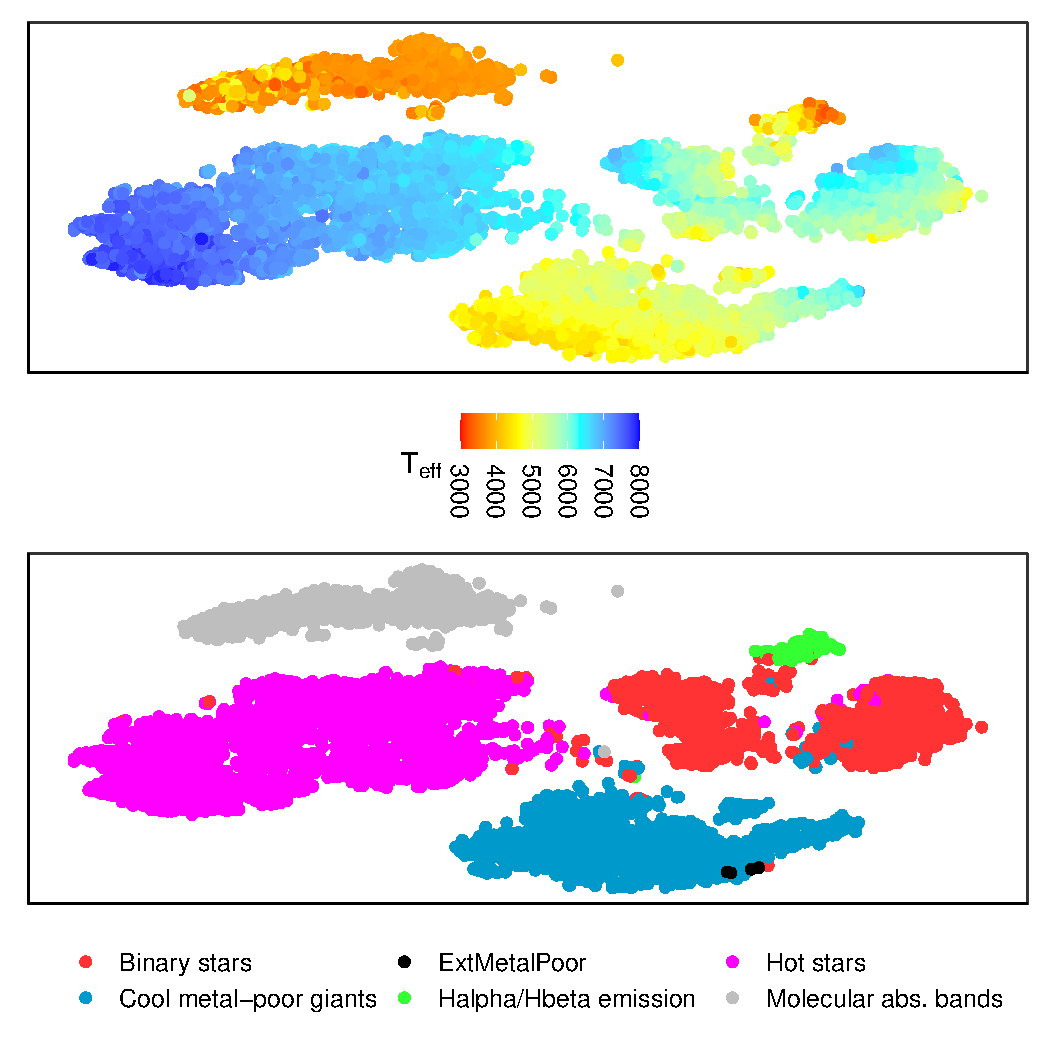
\includegraphics[width=\linewidth]{Plots/Figure1.pdf}
\caption{Illustrative \ts \ maps constructed only using the labelled portion our dataset. Top panel is coloured by effective temperature from \g DR3. Bottom panel the \ts \ map is coloured by stellar classification labels. 
Each point represents a star which has had its spectral information collapsed into two points in a 2-dimension parameter space produced by \ts; the axes are in arbitrary units reflecting only the dynamic range of the data in this space. 
Comparing the two panels shows that \ts \ is sensitive to effective temperature and the stellar classification. 
Note that neither spectroscopic temperature or classifications were included in the {\em input} to \ts.}
\label{fig:Classification}
\end{figure*}



	
\section{Method}\label{Sec:Method}	
Here we discuss a methodology that can be used to identify \emps \ within \g \ data, but also potentially adapted to find any stellar type within a given spectroscopic dataset. The methodology is a hybrid of machine learning and a more traditional model-fitting approach. Section~\ref{sec:Identification} outlines how to identify similar stars using a branch of machine learning known as dimensionality reduction, with a focus on targeting \emps . Once candidate \emps have been found, Section~\ref{Sec:fitting routine} describes the estimation of their stellar parameters.


\subsection{Identifying Similar Stars}\label{sec:Identification}

Identification of \emps \ in spectroscopic surveys typically involves the fitting of select regions of an observed spectrum with a synthetic spectrum, employing a metric to define their similarity (usually \ci)


\emps \ have, however, a relatively featureless spectrum, where distinguishing the difference between a real spectral feature and the inherent noise is challenging. 
Similarly, the {\em synthetic} spectrum of a metal-poor star is close to featureless, but lacks the noise that is present in an observed spectrum. Hence when applying a \ci-fitting method which entails comparing an observed spectrum with a synthetic spectrum, we expect stars that aren't extremely metal-poor to be identified as such (and vice-versa) due to model systematics. Ideally we would like a method that can 1) be independent of synthetic templates, 2) self-identify important features of a spectrum and 3) categorise similar spectra. 

To be able to create a method as described above is challenging for metal-poor stars. If, however, we could visualise the similarity of objects within a dataset, and group them visually, then we could reduce the search space for finding objects of interest, prior to running a \ci-fitting method. Furthermore, if we had a sample of the objects we were trying to identify, we could flag these before running a visualisation technique and see which groups they are clustered in, and hypothesise that the surrounding group must contain similar observations.
By approaching finding similar objects this way, we remove the necessity for synthetic template comparison at the identification phase of the process, resulting in a purer candidate sample.

Dimensionality reduction techniques, a branch of machine learning, are a standard way of extracting important features from large datasets.
Dimensionality reduction is the process of representing a high-dimensional data set $X={x_{1}, x_{2},\ldots,x_{N}}$, by a set $Y$ of vectors $y_{i}$ in two or three dimensions, and then placing similar observations in close proximity in the new parameter space, $y_{i}$, while keeping dissimilar observations at larger distances. The resulting reduced parameter space, $Y$, may then be visualised to determine similar and dissimilar input data.
The most common dimensionality reduction techniques used in astronomy are principal component analysis (PCA) and multidimensional scaling (MDS). Principal component analysis has been used by \cite{yip_2004} to classify quasars using SDSS spectral data; \cite{connolly_1999} demonstrated that PCA can be used to build galaxy SED's from data that may be noisy or incomplete; and \cite{fioren_2007} showed that PCA can be used to estimate stellar atmospheric parameters with SDSS/SEGUE spectra and \citet{2012MNRAS.421.1231T} used PCA to explore the stellar chemical abundance space. The frequent use of PCA underscores the importance of dimensionality reduction in the area of classification. 

A significant weakness in PCA, however, is that it is intrinsically linear. PCA does not consider the structure of the manifold; there may be data points that form a nonlinear manifold, which PCA will not be able to deconstruct. 
In addition, while dimensionality reduction techniques have been used in astronomy before, they generally were applied to smaller datasets. The effective parameter space for the \g \ data is 4 channels $\times$ 4096 pixels $\times$ 65,536 flux levels $\times$ 600,000 stars $\simeq 6 \times 10^{14}$ values; with a dataset of this magnitude, traditional techniques face a computational challenge.



\subsubsection{\ts}

Like other dimensionality-reduction techniques, \ts \  \citep{maaten_visualizing_2008} can be used to visualise how similar points are within a dataset.
\ts \ assesses the similarity of features in the higher-dimensional space by using the Euclidean distance metric (alternative metrics may be applied). A similarity matrix of probabilities, representing the higher-dimensional space, is calculated by converting these Euclidean distances using a standard Normal distribution. The feature space is then reduced to 2 or 3 dimensions, and the process above is repeated for this lower dimensional space; however, the t-distribution is used instead of a standard Normal distribution to construct the similarity matrix. To finally determine the lower dimensional representation of distances within our dataset, the Kulback-Leibler (KL) divergence between the two joint probability distributions is minimised using gradient descent. We chose the Barnes-Hut gradient descent version of t-SNE, implemented in the R package Rtsne\footnote{\url{https://github.com/jkrijthe/Rtsne}} by \citet{Rtsne}, as it substantially speeds up \ts \ and  allows \ts \ to be applied to much larger datasets that would be computationally intractable with the original \ts \ algorithm.
\ts \, unlike techniques such as PCA, is able to produce more visually compelling clusters because \ts \ 's non-linearity enables it to maintain the trade-off between local and global similarities between points. This makes \ts \ well suited to the purpose of finding and visualising the distribution of similar spectra in a large dataset.
Refer to \cite{traven_galah_2017} for a more detailed description of the t-SNE algorithm.

To illustrate the effectiveness of \ts \ at classifying stars using only their spectra, we  consider our defined labelled dataset of 9058 classified stars. For this application, only the spectral data for the labelled stars was passed in to \ts. The labels and additional stellar parameter information were not used. \ts \ 's input is a set of $9058 $ high-dimensional objects $x_{i}.... x_{N}$, where each object is described by 12288 wavelength values (for this analysis we ignore the infrared channel), representing a single star.
 Top panel of Figure~\ref{fig:Classification} shows the \ts \ map coloured by effective temperature ([$\mathrm{T_{eff}}$]). Bottom panel of Figure~\ref{fig:Classification} is the same map coloured by the classification labels in \cite{traven_galah_2017}. In both panels, the cluster of hot stars is clearly distinguishable by both temperature and label, highlighting that by applying \ts \ to only spectra, we can visualise sensitivity in both the stellar parameter and  stellar classification space.




\subsubsection{Determining which Wavelength Regions to Fit}\label{optimal_wavelength}

In searching for \emps it is important to understand the significant spectral features that are key indicators of extremely low metallicity. When dealing with low and medium-resolution spectra, traditionally the infrared calcium triplet or ultraviolet calcium H and K lines have been used as standard indicators of low metallicity.
These lines are, however, outside of the GALAH wavelength range.
Therefore the first step in applying our method to the entire \g \ dataset is to determine which metal lines within the \g \ wavelength range would be most useful for identifying \emps.



The optimal wavelength ranges were selected by determining the lower limit for \feh \ using the spectral templates. This was achieved by running a series of \ci \-fitting simulations using different elemental line combinations. The simulation which resulted in the highest level of certainty for the lowest \feh \ was selected. The optimal restricted wavelength ranges used are the regions around \Ha, \Hb , 4867-4872\AA \  and 4887-4892\AA \ ; the latter two ranges contain the strongest Fe I lines in the blue channel (4875.88\AA , 4890.76\AA\ and 4891.49\AA). Additionally we found that the OI triplet (7771.94\AA - 7775.39\AA) in the IR channel was a useful discriminant for removing hot stars that were contaminating the sample, and thus this range was also included.
In Figure~\ref{fig:sim_example} we show that, using spectra in the GALAH wavelength range, we can say with reasonable confidence that a star has a metallicity as low as \feh $\sim -3.5$ (or potentially below that value); see Appendix~\ref{deriving lines} for further details. 


By applying a method like \ts \ the idea is to reduce any bias that may arise in choosing which wavelength ranges to consider, as the technique may be able to better identify significant wavelength ranges not considered. 
To use the entire wavelength range, however, is a) computationally unfeasible and b) given the relatively featureless nature of \emp spectra, can introduce noise that may skew the final results.
We were thus unable to avoid having to select which wavelength ranges to input into \ts.




\subsection{Estimating Stellar Parameters for \emps }\label{Sec:fitting routine}

To confirm the identification of any EMP candidate found using the \ts \ methodology outlined in Section~\ref{sec:Identification}, we require an estimation of their basic stellar parameters, \teff, \logg \ and \feh.
The GALAH DR3 pipeline provides measurements of these stellar parameters for many of our candidates; however the DR3 pipeline is not tailored towards metal-poor stars with weak metal-lines.
We developed a simple iterative procedure to estimate each stellar parameter for a candidate EMP star, which is described below (see Section~\ref{Sec:Estimating stellar parameters of the cluster} for the application).


\begin{figure}
    \centering
    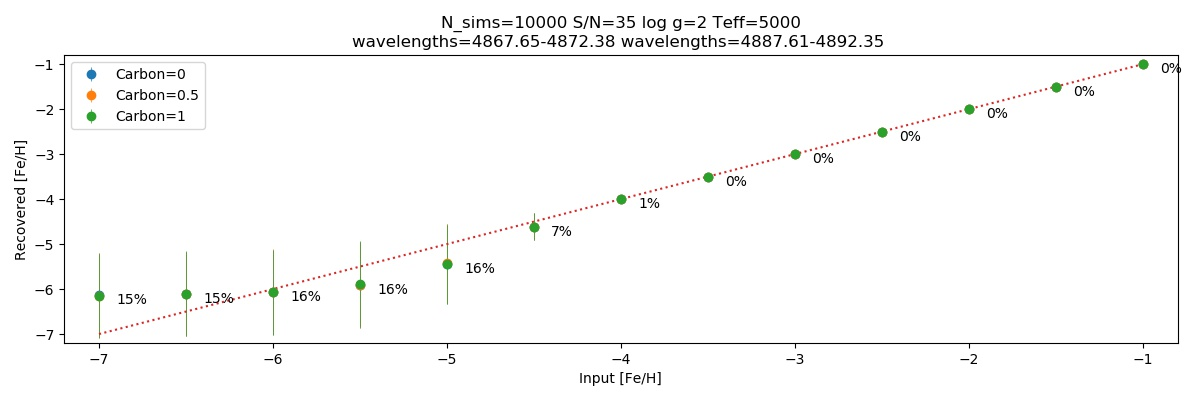
\includegraphics[width=\linewidth]{Plots/sim_plots/Nsim10000_SN35_logg2_T5000_Thomas_4870_4890.jpg}
    \caption{The output of a simulation fitting synthetic spectra with templates, showing that, given these stellar and observational parameters (\logg = 2, \teff = 5000K, S/N = 35) we can reliably estimate metallicities down to \feh $\lesssim -3.5$ with GALAH data. Percentages indicate fractional uncertainty from scatter in the recovered metallicities rounded to the nearest percentage. Due to the relative insensitivity to carbon in the GALAH wavelength ranges, the blue and orange points are masked by the green points. See Appendix~\ref{deriving lines} for further details. }
    \label{fig:sim_example}
\end{figure}


\begin{figure}
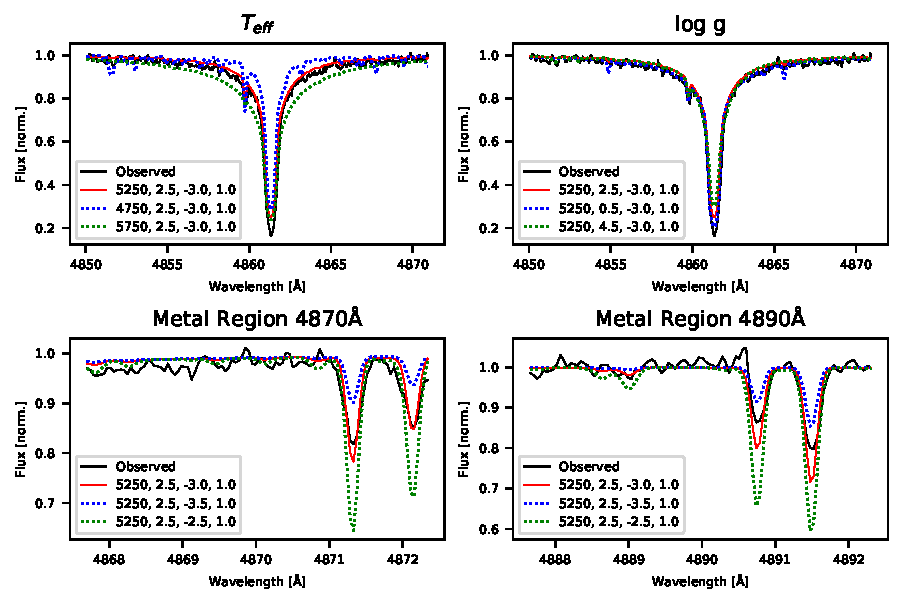
\includegraphics[width=\linewidth]{Plots/Figure3.pdf}
\caption{Fitting the observed \Hb \ region for a given star with the wider synthetic template grid as a test of the fitting of the stellar parameters, \teff, \logg and \feh. It is clear from the upper panels that this star is best fit by  a \teff \ of 5250 and a \logg \ of 2.5. The bottom panels represent the line regions considered in fitting \feh, and show that this star likely has a metallicity \feh between -3.0 and -3.5. The parameters of the synthetic templates as given in the panels are \teff, \logg, \feh and [C/Fe] (the assumed [C/Fe] may be ignored for these fits).} 
\label{fig:parameter_fits_teff_logg}
\end{figure}



\subsubsection{Effective Temperature, Surface Gravity and Metallicity }\label{Fitting teff}

To estimate \teff \ , \logg \ and \feh, we apply a \ci-minimisation routine between the observed spectra and the synthetic templates defined in Section~\ref{sec:synths} using only the \Ha \ and \Hb \ regions and a select few metallicity lines around 4870\AA \ and 4890\AA . We fit the lines simultaneously to account for the degeneracies that arise between the stellar parameters, and select the template corresponding to the minimum \ci.



The upper half of Figure~\ref{fig:parameter_fits_teff_logg} shows the fitting of the \Hb \ region to 3 synthetic templates for a given star, with the optimal fit of \teff \ equal to 5250, shown in red, and the best fit of \logg \ as 2.5.
The bottom panels of Figure~\ref{fig:parameter_fits_teff_logg} show the two line regions considered in the fitting of metallicity, which suggest this observed star may have a metallicity in the range $-3.5 <$ \feh $< -3.0$.



\begin{figure*}
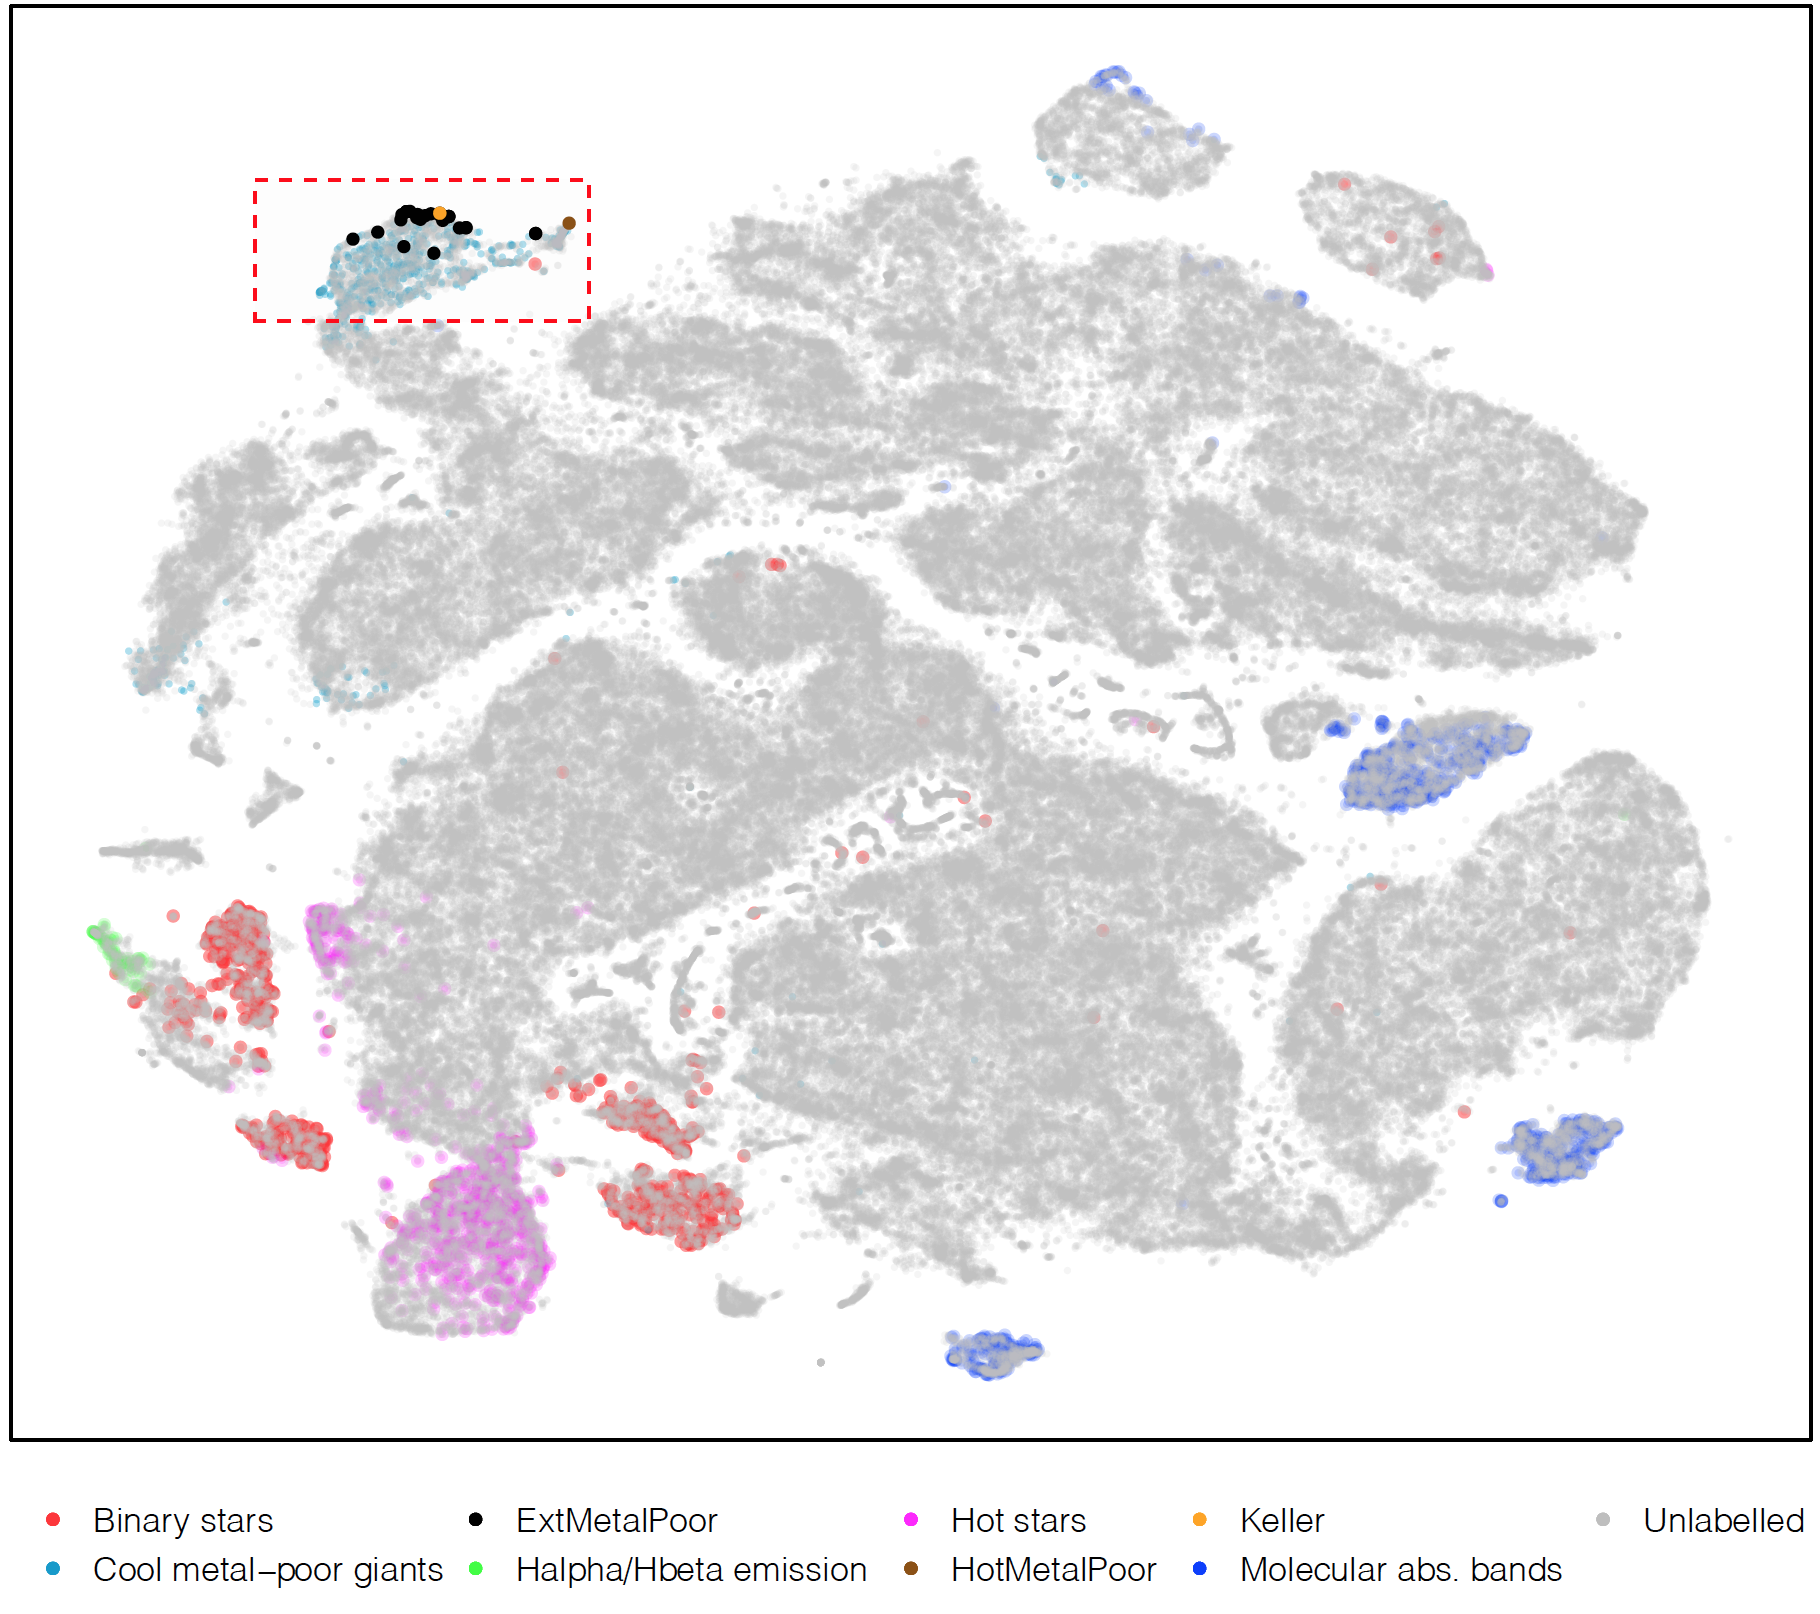
\includegraphics[width=\linewidth,keepaspectratio]{Plots/Figure4.png}
\caption{t-SNE map with the unknown (unlabelled) stars plotted in grey and the known extremely metal-poor stars -- corresponding to the stars shown in Table~\ref{tab:Metal-Poor_Table} -- overlaid in black, brown and orange. A region containing all 5 (*) stars and the additional known metal-poor stars is located to the top left of the map. The dashed box represents the ``island" selected for  further analysis, with the extremely metal-poor stars focused on the upper `coast' of the island.}
\label{fig:tsne_map}
\end{figure*}



\section{Results}\label{Sec:Results}

The following section describes the results of applying the outlined methodology to the full \g \ dataset inclusive of unclassified stars, as defined in Section~\ref{sec:sample selection}. Section~\ref{Sec:Application} applies our hybrid \ts \  methodology, Section~\ref{Sec:Estimating stellar parameters of the cluster} and Section~\ref{Sec:Candidates} estimates the stellar parameters and applies some further analysis on the candidate sample.




\subsection{Applying the \ts \ methodology}\label{Sec:Application}

\begin{figure*}
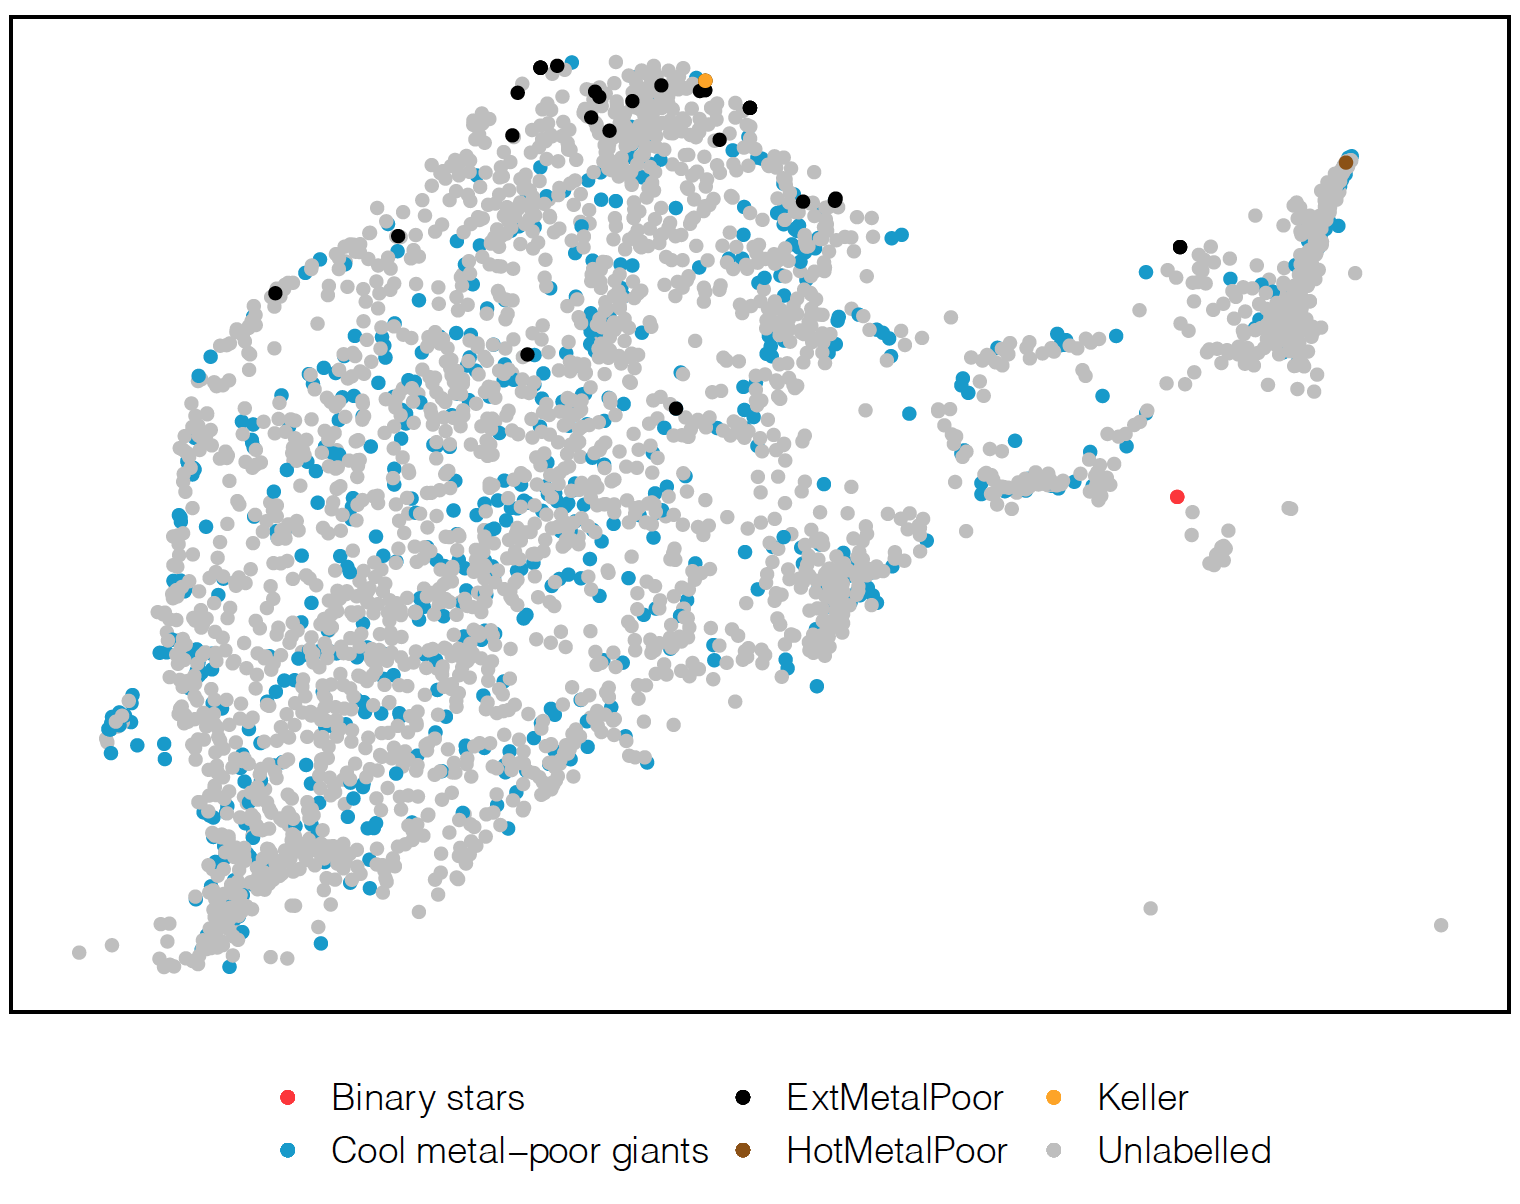
\includegraphics[width=\linewidth,keepaspectratio]{Plots/Figure5.png}
\caption{A zoomed in view of the island highlighted by the red-dashed box in Figure~\ref{fig:tsne_map} with 2487 potential metal-poor stars. The known \emps \ lie on the upper extremely metal-poor ``coast" of the island.}
\label{fig:tsne_map_zoomed}
\end{figure*}

Applying the methodology to find \emps \ described in Section~\ref{sec:Identification}, we consider the entire GALAH sample, subsetted by the optimal wavelength regions as determined in \ref{optimal_wavelength} and with the \emps \ and the Keller star flagged. We will use the additional classification labels defined in Section~\ref{sec:stellar labels}, to flag other structures in the \ts \ plane.

The \ts \ method was calculated with the perplexity set to 40, the number of iterations set to 2000 and the other hyperparameters (see \cite{wattenberg_how_2016}) left to their default values.
The processing was run on an Ubuntu server, with 344GB of RAM and an Intel Xeon CPU E5-2695 v3 @ 2.30 GHZ with 30 threads.

The resulting map is shown in Figure~\ref{fig:tsne_map}.
A separate ``island'' containing all 5 known \emps \ and the Keller star is located in the top left of the map.
We infer that the unlabelled stars surrounding the known Keller and \emps \, form a potential metal-poor cluster on the map. This cluster is then extracted and passed into our stellar parameter fitting routine described in Section~\ref{Sec:fitting routine}, reducing the search space to fit stellar parameters of potential \emps \ from 600,000 to approximately 2500. A zoomed in image of this cluster is shown in Figure~\ref{fig:tsne_map_zoomed}.



\begin{figure*}
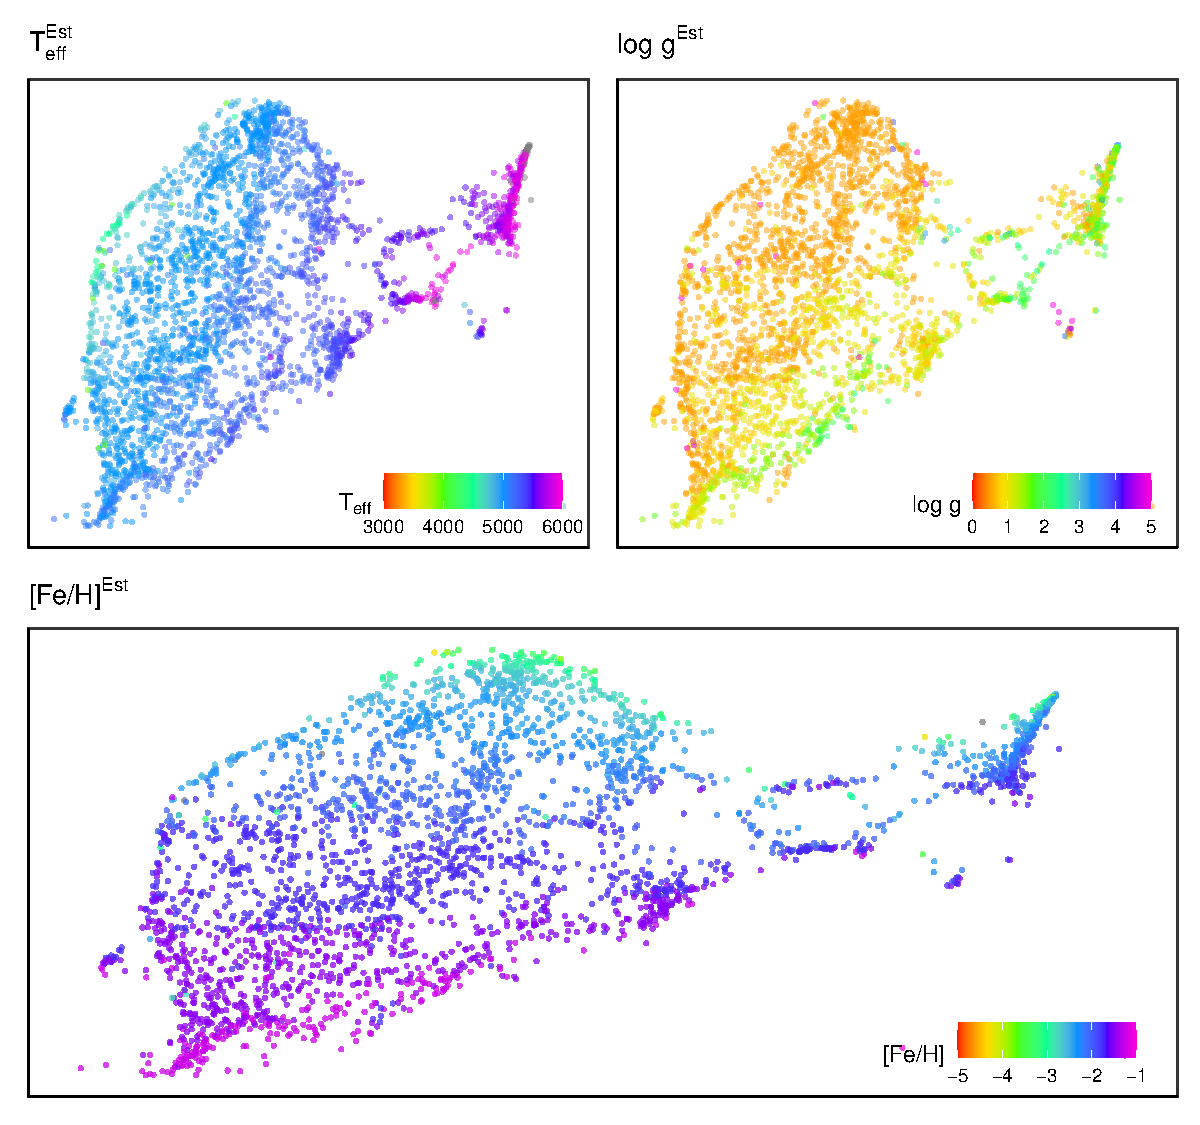
\includegraphics[width=\linewidth,keepaspectratio]{Plots/Figure6.pdf}
\caption{Three panels showing the selected island coloured by each stellar parameter. The top-left panel shows our estimated \teff, having a distribution of temperature from cold to hot going left to right. Similarly the top-right panel shows estimated \logg \ having a similar left to right distribution. The lower panel shows estimated \feh \ having a gradient of high to low metallicity from bottom to the top, with the top edge in agreement with the previously seen ``extremely metal-poor coast". }
\label{fig:estimate_elephants}
\end{figure*}




\subsection{Stellar Parameter Estimation for the \emps \ Cluster }\label{Sec:Estimating stellar parameters of the cluster}
Taking the hypothesised metal-poor only island, we estimate the stellar parameters for each star in the island using our simple stellar parameter fitting routine described in Section~\ref{Sec:fitting routine}.

The estimated \teff \ and \logg \ values for our  metal-poor island are shown in the upper two panels of Figure~\ref{fig:estimate_elephants}. Here we see a similar distribution of \teff and \logg, with cooler giant-type stars on the left, going to hotter, higher \logg stars to the right of the island.
\feh \ is shown in the bottom panel of Figure~\ref{fig:estimate_elephants} and displays a gradient of metallicity, higher to lower, from the bottom to the top edge of the island. The previously defined extremely metal-poor coast (as seen in Figure~\ref{fig:tsne_map_zoomed}) is evident. 



Before identifying and analysing EMP candidates in our cluster, we note that our stellar parameter fitting routine is relatively simple and is only used as a guide. The method was necessary, as we see a significant scatter with respect to DR3 pipeline-derived metallicities, as well as a systematic tendency toward higher measured metallicities in DR3. This may be attributed to the GALAH analysis pipeline being optimised for thin and thick disk stars, with typical metallicities \feh $\geq -2$. Moreover, a comparison of our metallicity estimates for the stars with both the (admittedly heterogeneous) literature metallicities and \g DR3 metallicities, shown in Figure~\ref{fig:Fehlit}, suggests that our method is yielding reasonable estimates for \feh. Similar comparisons for our estimates of \teff and \logg (Figures~\ref{fig:Tefflit} and \ref{fig:Logglit}, respectively) also show acceptable agreement with values from both the literature and \g DR3. 

\begin{figure}
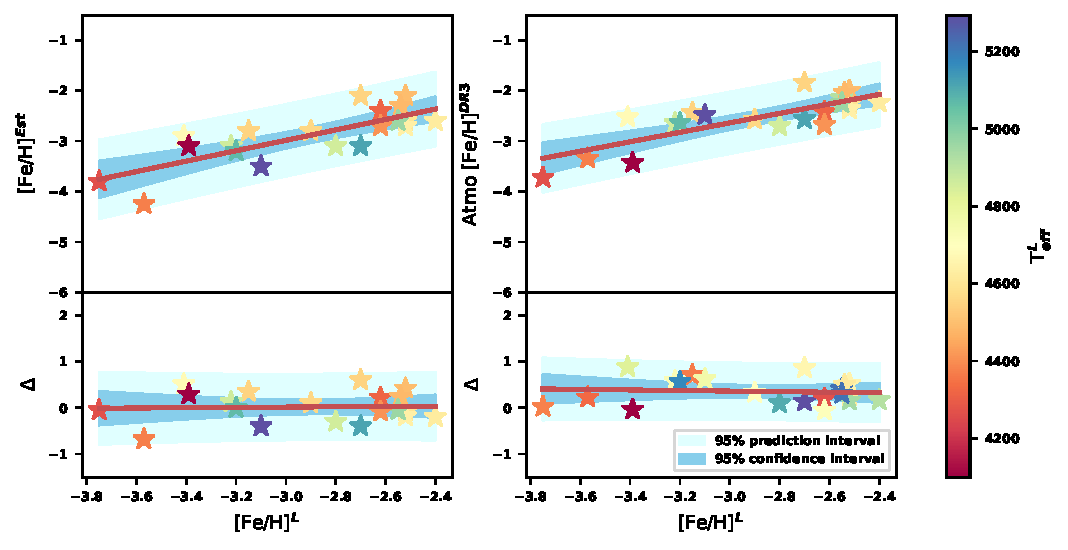
\includegraphics[width=\linewidth,keepaspectratio]{Plots/Figure7.pdf}
\caption{Two plots comparing our estimated \feh \ (left) and GALAH DR3  \feh (right) \ values with the literature. The top panels show the respective values while the bottom panels represent the difference between the method/s and the literature. The red line shows a linear best-fit to the data, with the prediction and confidence intervals as indicated by the shaded regions. Overall both methods have a 95\% confidence band of approximately $ \mathrm{\pm 0.5}$ but the GALAH DR3 measured \feh \ values are higher on average than literature metallicities in this low-metallicity range.}
\label{fig:Fehlit}
\end{figure}



\begin{figure}
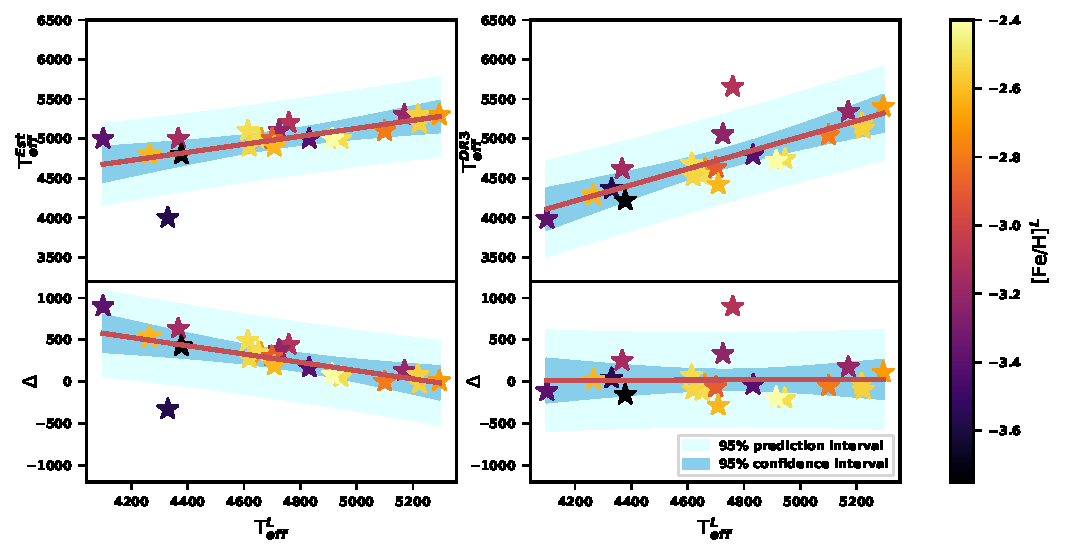
\includegraphics[width=\columnwidth,keepaspectratio]{Plots/Figure8.pdf}
\caption{Two plots comparing our estimated \teff \ (left) and GALAH DR3 \teff \ (right) with the literature. The top panels show the respective values while the bottom panels represent the difference between the method/s and the literature. The red line shows a linear best-fit to the data, with the prediction and confidence intervals as indicated by the shaded regions.  There is a trend in the errors of our estimation method, in that we have higher \teff \ at the lower end but overall have a similar error band to that of GALAH DR3.}
\label{fig:Tefflit}
\end{figure}


\begin{figure}
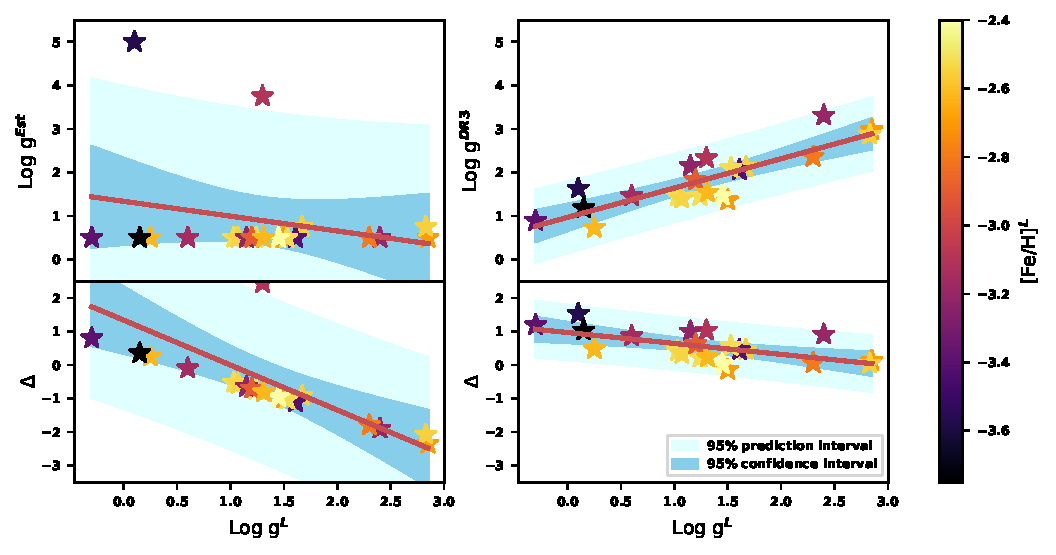
\includegraphics[width=\linewidth,keepaspectratio]{Plots/Figure9.pdf}
\caption{Two plots comparing our estimated \logg \ (left) and GALAH DR3 \logg \ (right) values with the literature. The top panels show the respective values while the bottom panels represent the difference between the method/s and the literature. The red line shows a linear best-fit to the data, with the prediction and confidence intervals as indicated by the shaded regions.  Here you can clearly see that the GALAH DR3 estimates of \logg \ are a much better match, which is to be expected, given the relative simplicity of our method. }
\label{fig:Logglit}
\end{figure}












\begin{sidewaysfigure}
\includegraphics[scale=0.4,keepaspectratio]{Plots/Figure10.png}
\caption{A candidate from the \ts EMP island identified in Figure~\ref{fig:tsne_map_zoomed} plotted over the 4 GALAH wavelength ranges, and overlaid with the best synthetic spectrum match in red, as well as a vertically-shifted comparison spectrum offset by +1.0 in \feh \ shown in blue. The best-fit stellar parameters are listed in the bottom-right inset table and the vertical dashed lines represent the different wavelength regions used, as defined in Section~\ref{optimal_wavelength}.}
\label{fig:prime_candidate}
\end{sidewaysfigure}

\subsection{Candidates}\label{Sec:Candidates}
Having used the template fitting process described in Section~\ref{Sec:fitting routine} to estimate the stellar parameters of our cluster in Section~\ref{Sec:Estimating stellar parameters of the cluster}, we find 380 stars that have \feh \ $\leq-2.5$ and 135 stars with  \feh \ $\leq-2.7$. For the rest of the discussion, however, we only consider stars that have \feh \ $\leq-3$, to satisfy the ``extremely" metal-poor star designation. 
This results in 54 EMP candidates,  6 of which have an estimated \feh $\leq-3.5$.
We note that 9 SIMBAD-sourced \emps from the literature in Table~\ref{tab:Metal-Poor_Table} are all contained in this \ts \ sample, and 7 (2 of which overlap with the literature) were identified as potential \emps by the GALAH DR3 pipeline, resulting in a net total of 40 potentially previously unidentified candidate EMP stars.



\begin{table}[]
\scalebox{1.0}{
\centering
\begin{tabular}{llllll}
\hline
{\tt s\_object\_ID}     & {\tt RA} & {\tt DEC}  &        $\mathrm{T^{Est}_{eff}}$ &
  $\mathrm{log \ g^{Est}}$ &
  $\mathrm{[Fe/H]^{Est}}$    \\
\hline
\hline
131123002501215 & 63.5677656 & -60.151311 & 5000 & 0.50 & -3.00 \\
131217002301168 & 64.8334861 & -58.678350 & 5200 & 0.50 & -3.10 \\
140312003501132 & 203.154833 & -38.009181 & 4900 & 0.50 & -3.30 \\
140711001301222 & 242.630802 & -25.337563 & 5000 & 0.50 & -3.20 \\
140808004701080 & 28.0619680 & -72.320519 & 5600 & 0.75 & -3.40 \\
140809004901060 & 40.9968414 & -70.248597 & 4000 & 5.00 & -3.00 \\
$\cdots$ & $\cdots$ & $\cdots$ & $\cdots$ &$\cdots$ & $\cdots$\\

\hline

\end{tabular}}
\caption{A subset of EMP candidates, with the full candidate list available electronically.}
\label{tab:Metal-Poor_Candidates}
\end{table}


The spectra of the 54 candidate \emps are relatively featureless (with the exception of \Ha \ and \Hb) across the HERMES wavelength ranges; Table~\ref{tab:Metal-Poor_Candidates} shows the derived parameters for a few of our candidates. The spectrum of a representative EMP candidate from our selection is shown in Figure 10. This star has an \feh$<-4.5$, as determined by our stellar parameter routine. 

As a first attempt for confirmation that the candidates are likely EMP stars, we display their photometric properties in a parameter space that has successfully been used to select \emps. Figure~\ref{fig:sky_mapper} shows our sample cross-referenced with the SkyMapper photometric catalogue \citep{2019PASA...36...33O}.
Here $m_{i}$ represents a metallicity index, defined
as $(v-g)_{0} - 1.5(g-i)_{0}$, and $(g-i)_{0}$, as a proxy for \teff. We show the EMP selection region in the figure from \citet{Da_Costa_2019}, and find that  most of our candidates are red giants and our sample fits within this region. 
This suggests, at least in terms of the broad metallicity-sensitive features targeted by the SkyMapper photometry, that our sample contain {\em bona fide} \emps. We note that \citet{Da_Costa_2019} find that $7\%$ of the stars within the SkyMapper selection region ultimately prove to be \emps based on follow-up spectroscopy. 



\begin{figure}
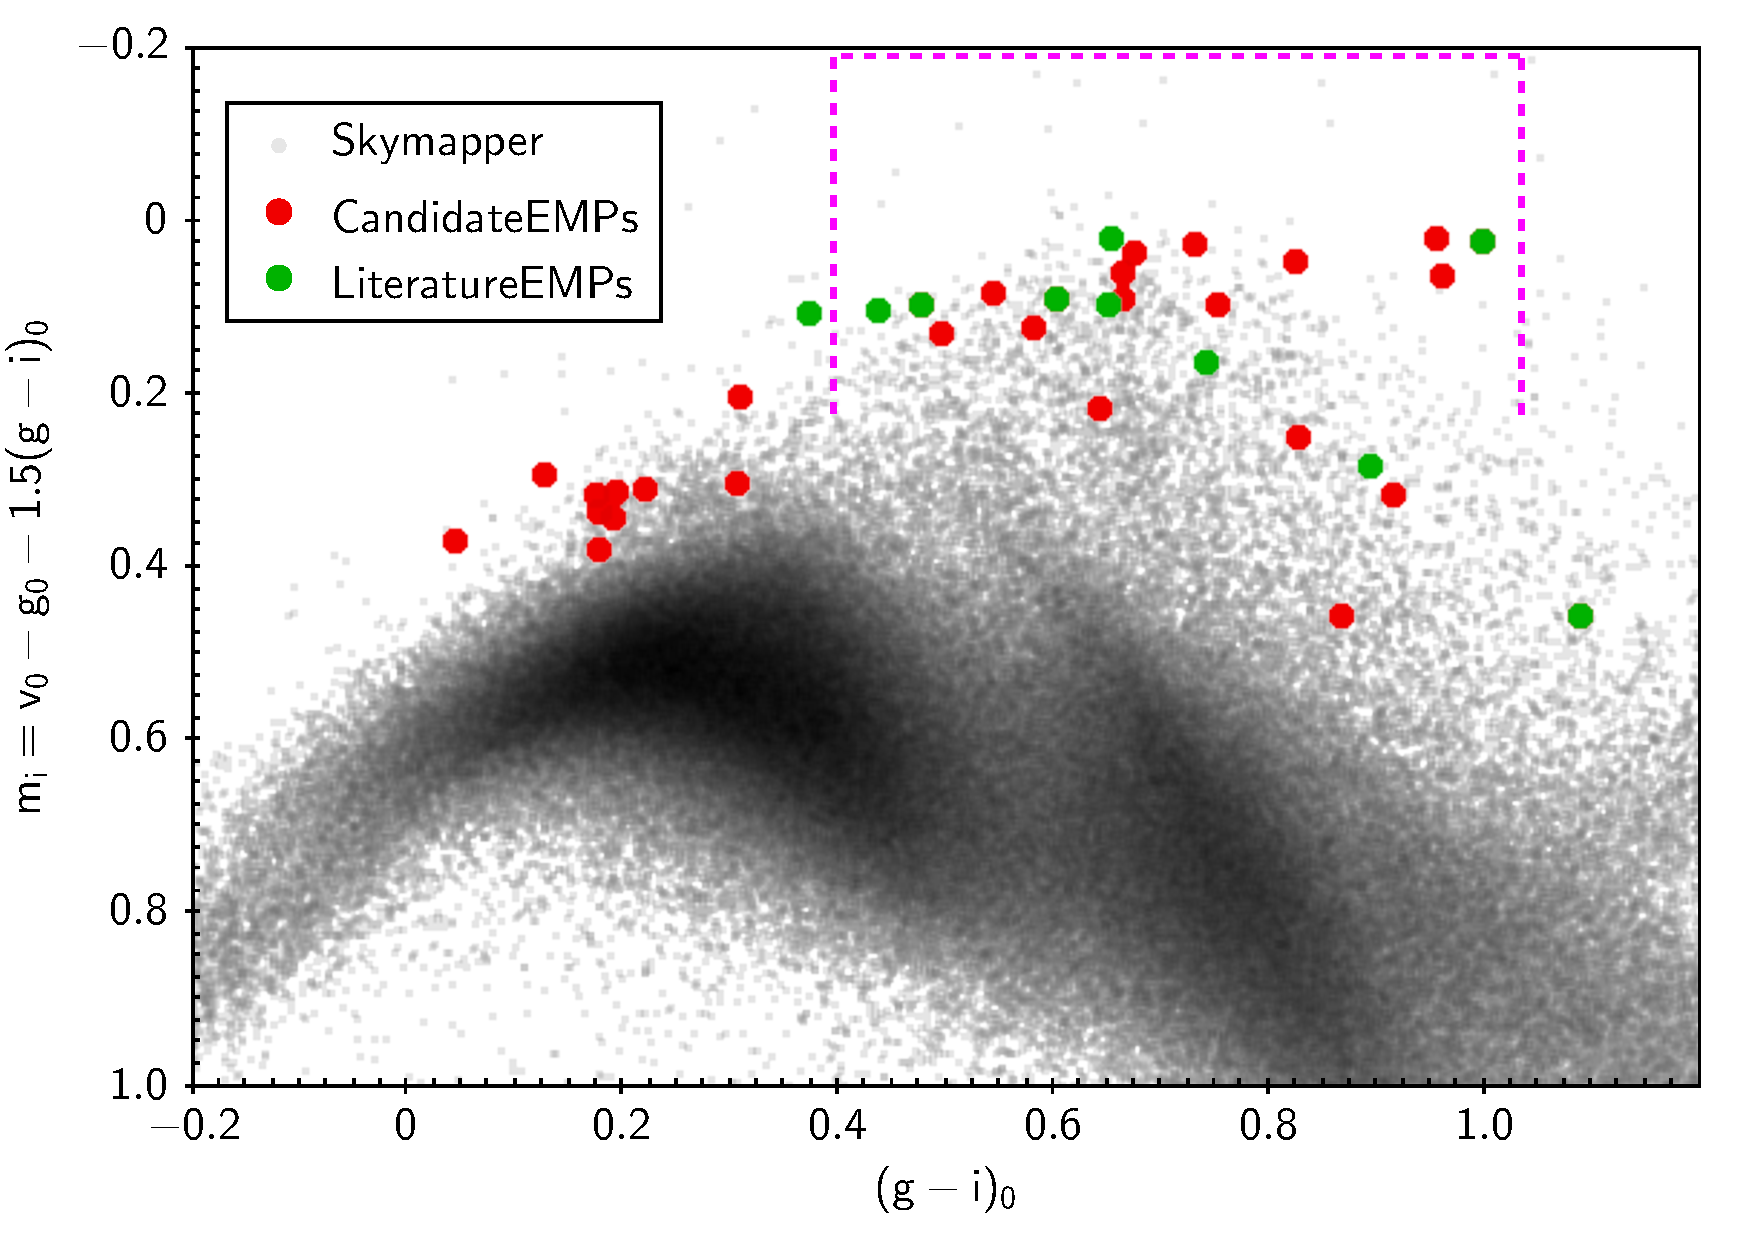
\includegraphics[width=\linewidth]{Plots/Figure11.pdf}
\caption{A Skymapper metallicity-sensitive diagram, showing most of our candidates are likely red giants falling within the SkyMapper selection window \citep[dashed magenta lines, from][]{Da_Costa_2019}. The compact grouping to the left represents candidate EMP main sequence turn-off stars.}
\label{fig:sky_mapper}
\end{figure}


What about the candidates that fall {\em outside} of that selection box? We plot our candidates and the known literature stars on a color-magnitude diagram, using {\tt pho\_g\_mean\_mag} and the color {$G_{BP} - G_{RP}$} from GAIA DR2 \citep{gaia_dr2}, and distances from GAIA \citep{2018AJ....156...58B} in Figure~\ref{fig:bird_plot}. The majority of our candidates fall on the red giant branch along with some literature \emps, suggesting they are mostly red giants. Some of our candidates, however, are located near the main sequence turn-off. A significant portion of our EMP candidates indeed show higher surface gravities, suggesting they are actually main sequence turn off stars.

\begin{figure}
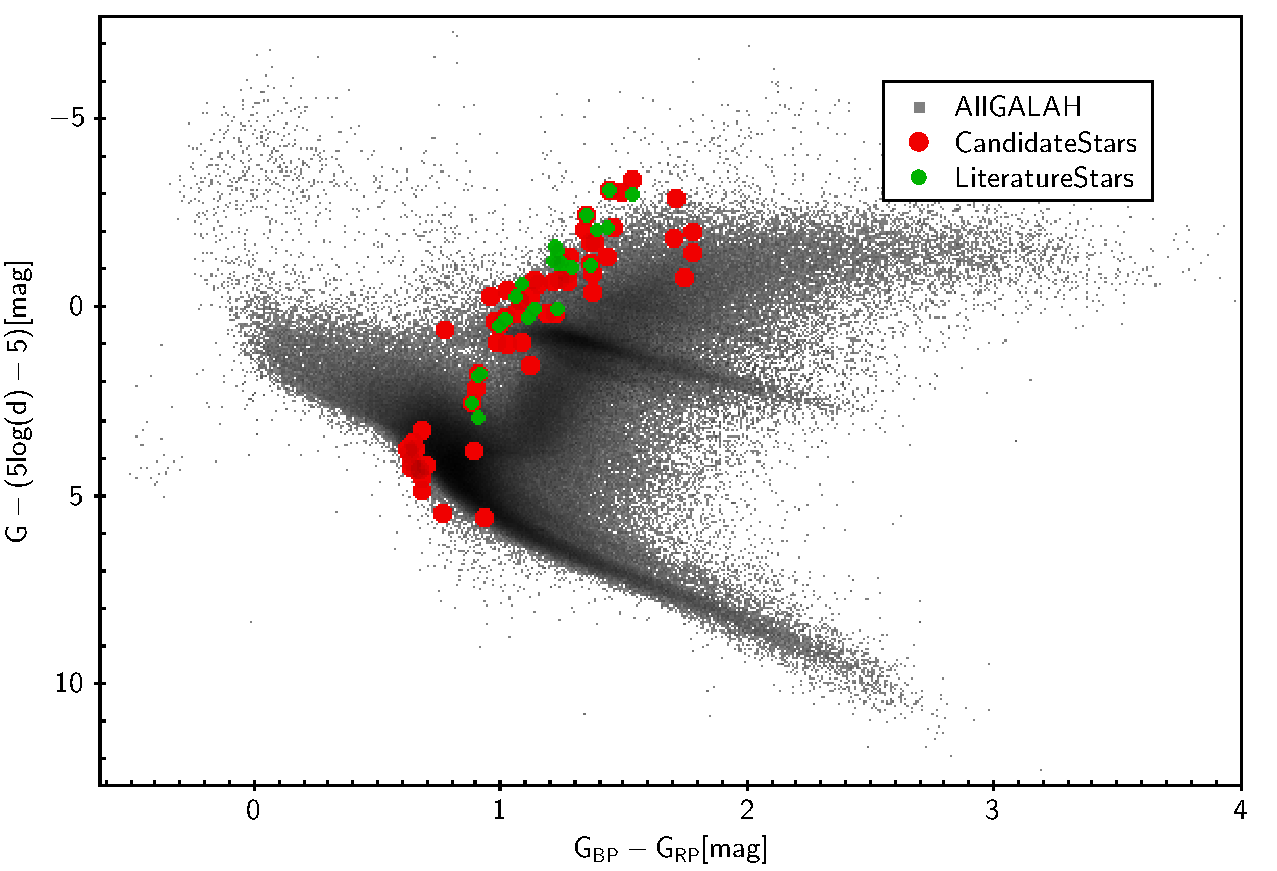
\includegraphics[width=\linewidth]{Plots/Figure12.pdf}
\caption{The color-magnitude diagram using magnitudes and distances from GAIA DR2 for the candidate EMP stars (yellow circles).The majority of the EMP candidates are red-giants, while 20\% appear to be consistent with main-sequence turn off stars. Green circles are known EMP stars as defined in Table~\ref{tab:Metal-Poor_Table}, including the most iron-poor star known, SMSS J031300.36–670839.3  \citep{keller_single_2014}.}
\label{fig:bird_plot}
\end{figure}





\section{Discussion}\label{Sec:Discussion}
At a high-level, given that we already had a large sample of high resolution spectra our candidate selection was relatively straightforward compared to previous EMP work: we have a magnitude-limited sample of stars and simply identified the population using iron and hydrogen absorption lines\footnote{As noted previously, we also used an oxygen feature, but only as a discriminant to remove hot stars that were contaminating the sample.}. We note this is only possible because, even with the relatively limited wavelength coverage of GALAH spectra, that there is still sufficient sensitivity to spectral features indicative of EMP-like metallicities (see Appendix~\ref{deriving lines}).

One question which arises is how our sample compares to previous work on the metallicity distribution function (MDF) for EMP stars. The topic has been explored in a number of recent studies \citep[e.g.,][]{DaCosta2019,2020MNRAS.492.4986Y, 2021MNRAS.507.4102Y}, with
\citet{2021MNRAS.507.4102Y} finding a slope for the MDF of $\mathrm{{\Delta(\log N)}/{\Delta[Fe/H] } = 1.51}$ dex per dex for $-4.0<$ [Fe/H] $<-3.0$, with an apparent steep drop-off below -4.0 (below -4.0 it would appear virtually all stars are C-enhanced, with the [Fe/H] values likely varying stochastically depending on Population III supernova yields).The left panel of Figure~\ref{fig:mdf} shows the MDF for our candidate sample and the right panel shows a log-scaled histogram with the gradient of 1.51 from \citet{2021MNRAS.507.4102Y} overlaid (red-dashed line).
Here we can see that the ``unbiased” nature of the current sample, which provides another way of investigating the form of the MDF, yields reasonably consistent results. However, given the MDF presented in \citet{2021MNRAS.507.4102Y}  and the current sample size (~50 stars with [Fe/H] $<-3.0$), the probability of any of the current EMP candidates having [Fe/H] $<-4.0$ is not very high, as most will be closer to -3.0. Hence a significantly larger EMP sample is required for probing the low-metallicity end of the stellar MDF; in this paper we have demonstrated that applying our approach to larger samples reaching fainter magnitudes is a key way to generate such an EMP sample.

\begin{figure}
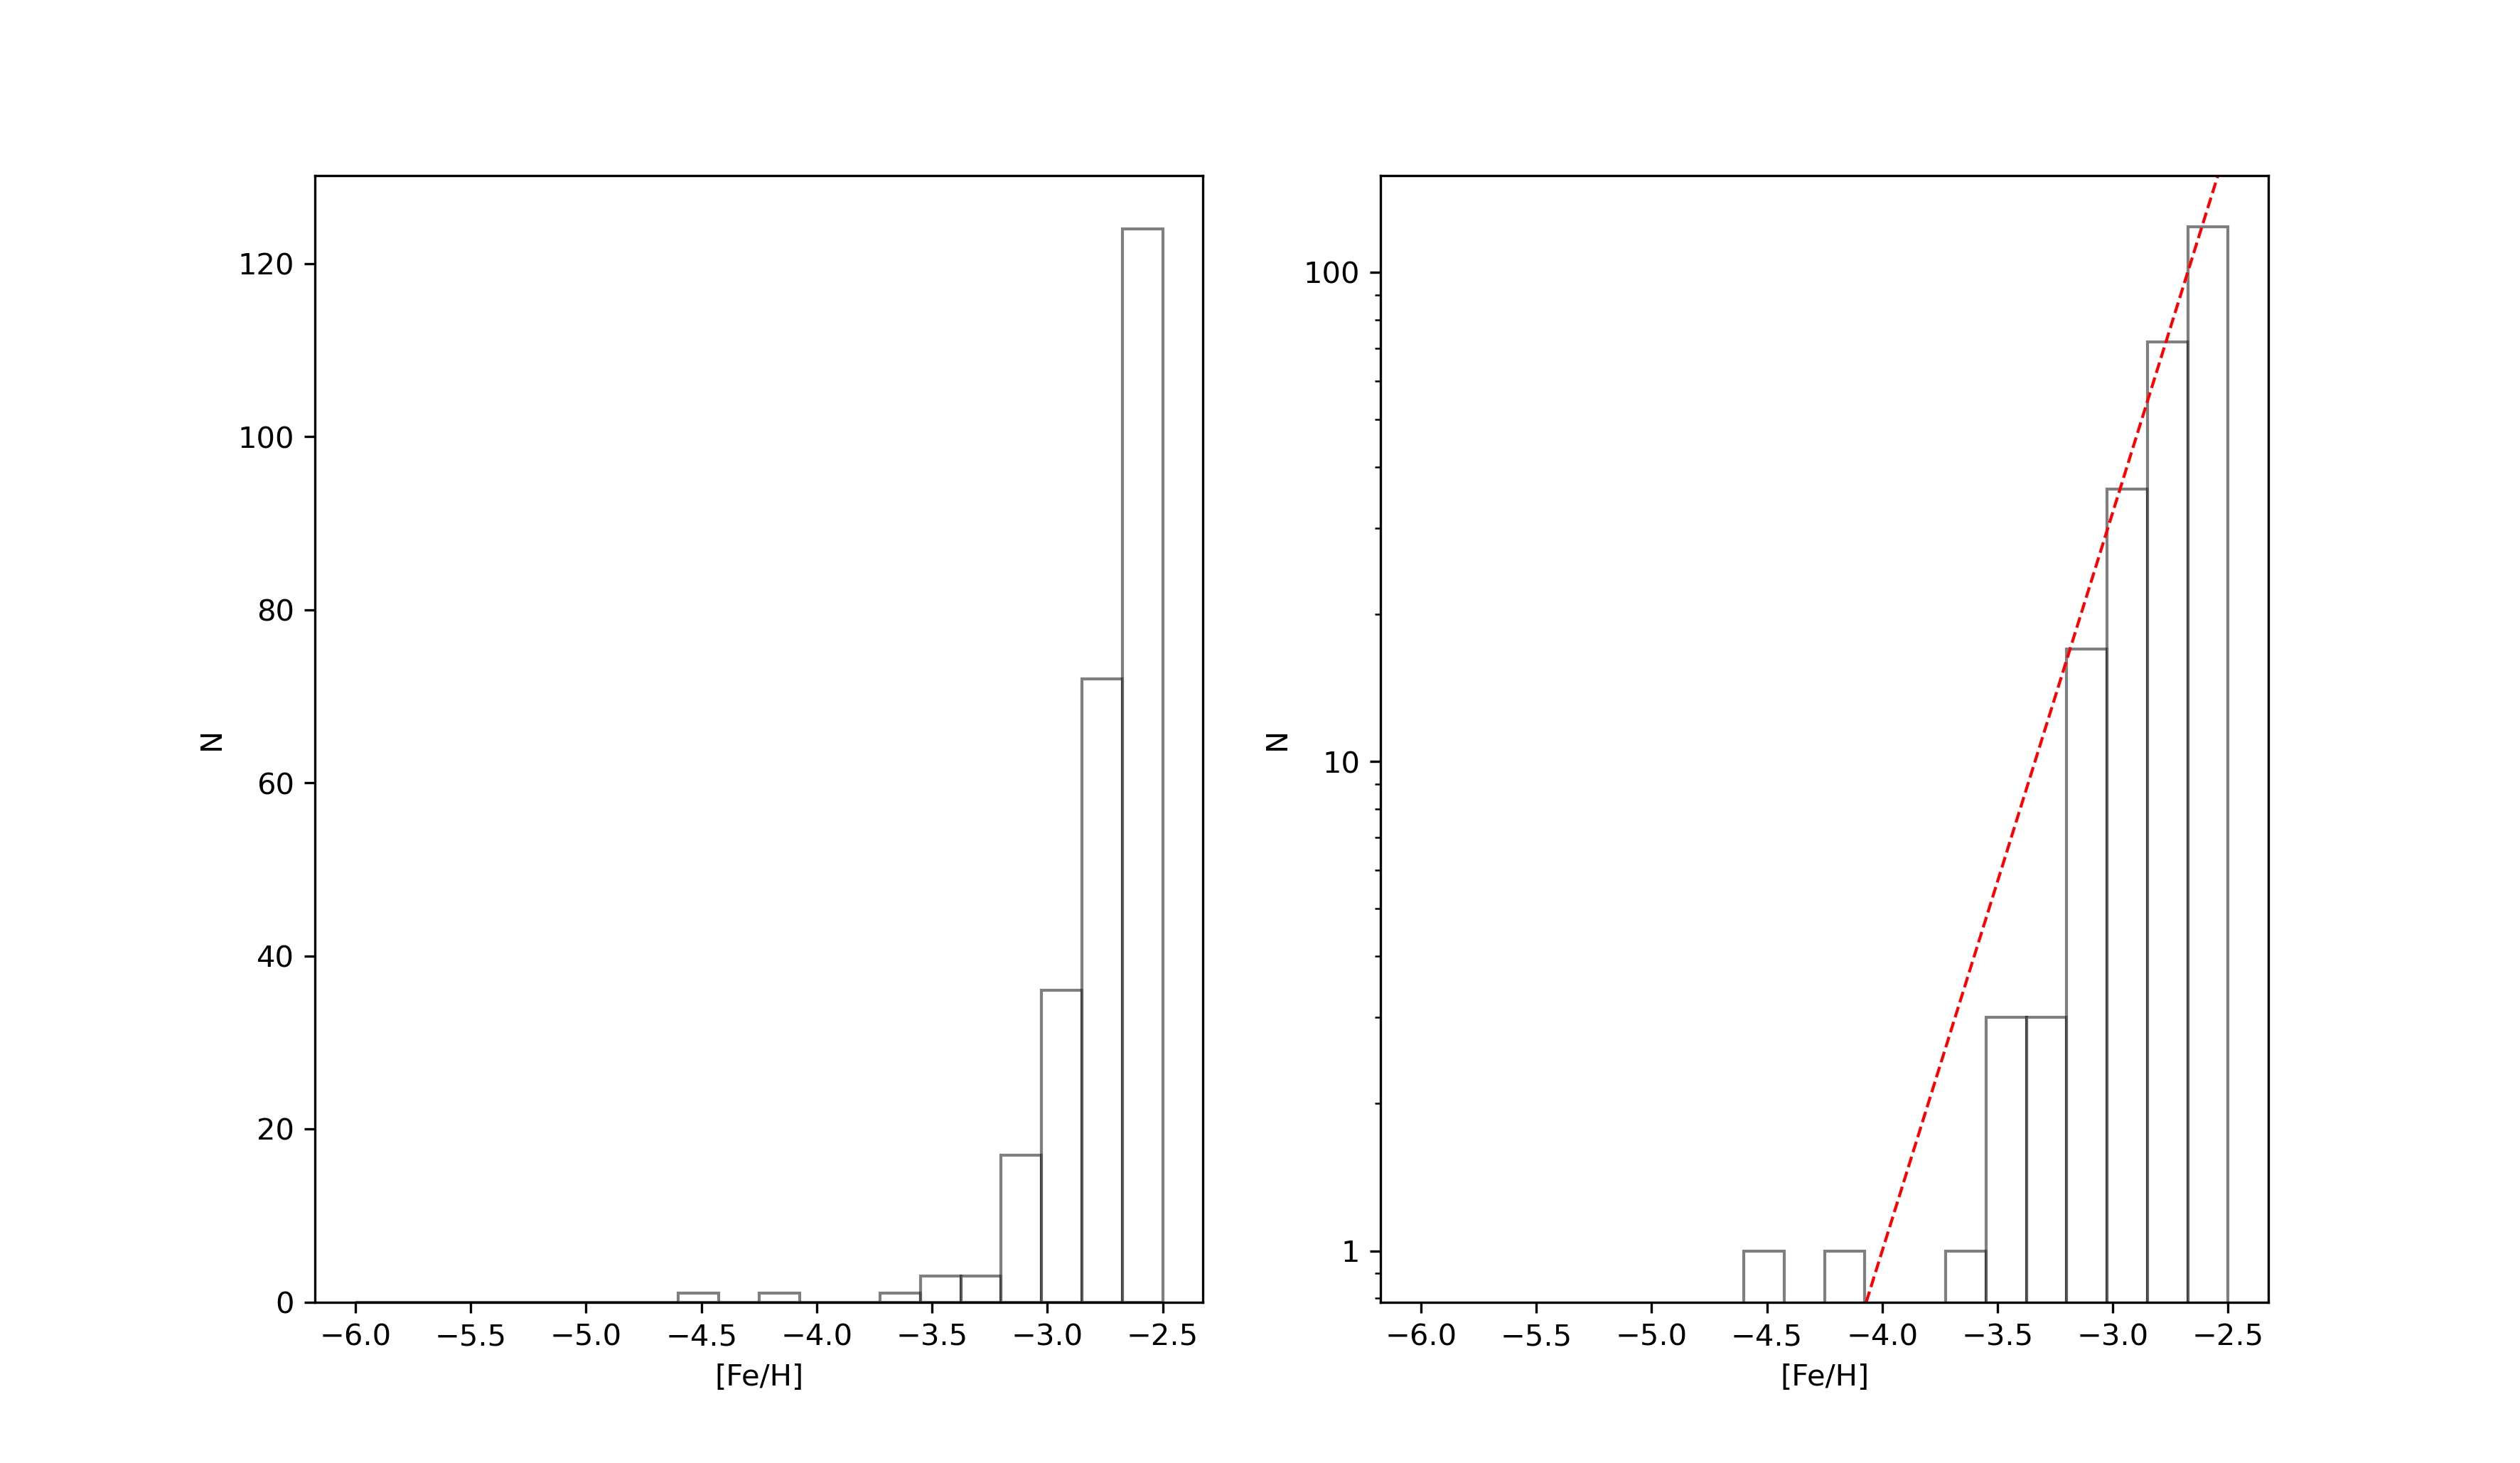
\includegraphics[width=\linewidth]{Plots/Figure13.png}
\caption{Metallicity distribution function for our candidate sample (left) and the log-scaled distribution function with the slope of 1.51 as determined in \citet{2021MNRAS.507.4102Y}  overlaid (red-dashed line). For this histogram we only show candidates from the main GALAH survey, which is a magnitude-limited sample. We specifically exclude stars in GALAH DR3 targeted by other surveys (K2-HERMES \cite{2018AJ....155...84W}, TESS-HERMES \cite{2018MNRAS.473.2004S} and GALAH-faint) because they incorporated fainter stars. The MDF follows a similar trend to that as seen in \citet{2021MNRAS.507.4102Y}, except for steeper fall-off at [Fe/H] $<-3.3$.}
\label{fig:mdf}
\end{figure}



Although the sample requires further spectroscopic observations to confirm our stellar parameter estimates, its relatively unbiased nature means there are a number of promising properties of the sample that suggest the method developed here has some advantages over other techniques for finding and understanding the EMP population.

Firstly, as shown in Figure~\ref{fig:sky_mapper} and Figure~\ref{fig:bird_plot}, we appear to have identified some main-sequence or main-sequence turnoff candidates. This is interesting because the sample of EMP stars from the literature observed serendipitously by GALAH (see e.g.Table~\ref{tab:Metal-Poor_Table}) consists of essentially all giant stars, reflecting the fact that previous work \citep[e.g.,][]{Starkenburg2017} prioritised probing larger volumes in order to obtain large samples of relatively rare EMP stars. For this reason most surveys specifically targeted stars with giant-like properties, whose high luminosities allow them to be studied at greater distances.

If even one of our main sequence EMP candidates turns out to be a {\em bona fide} main sequence or main sequence turn-off EMP star, this is an exciting opportunity to explore a less-studied population of \emps. The abundance patterns of main sequence stars are comparatively easy to understand because they have not yet been affected by evolution in the post main sequence phase. The ages of these stars are also more accessible through comparison to isochrones, which is important for placing these \emps into the context of the formation and assembly of the Milky Way.

Another advantage of our method, which differs from other EMP selection methods -- e.g., some combinations of photometric filters \citep{Da_Costa_2019} -- is that carbon features did not affect our candidate selection. This means we have a relatively unbiased sample with respect to carbon abundance. Carbon-enhanced metal-poor stars (which have [C/Fe] \textgreater~0.7), become increasingly more frequent as [Fe/H] decreases (e.g., \citealt{2014ApJ...797...21P}), and for [Fe/H]$\leq$ –4.0, carbon-enhanced metal-poor stars dominate the known sample. Hence this candidate sample presents an opportunity to explore the relative fraction of carbon-enhanced metal-poor stars as a function of [Fe/H] free of carbon-influenced selection bias. In fact, GALAH does not cover the wavelength ranges required to estimate carbon at extremely low metallicities, making follow-up observations of this magnitude limited candidate sample essential for studying its carbon abundances.

\begin{figure}
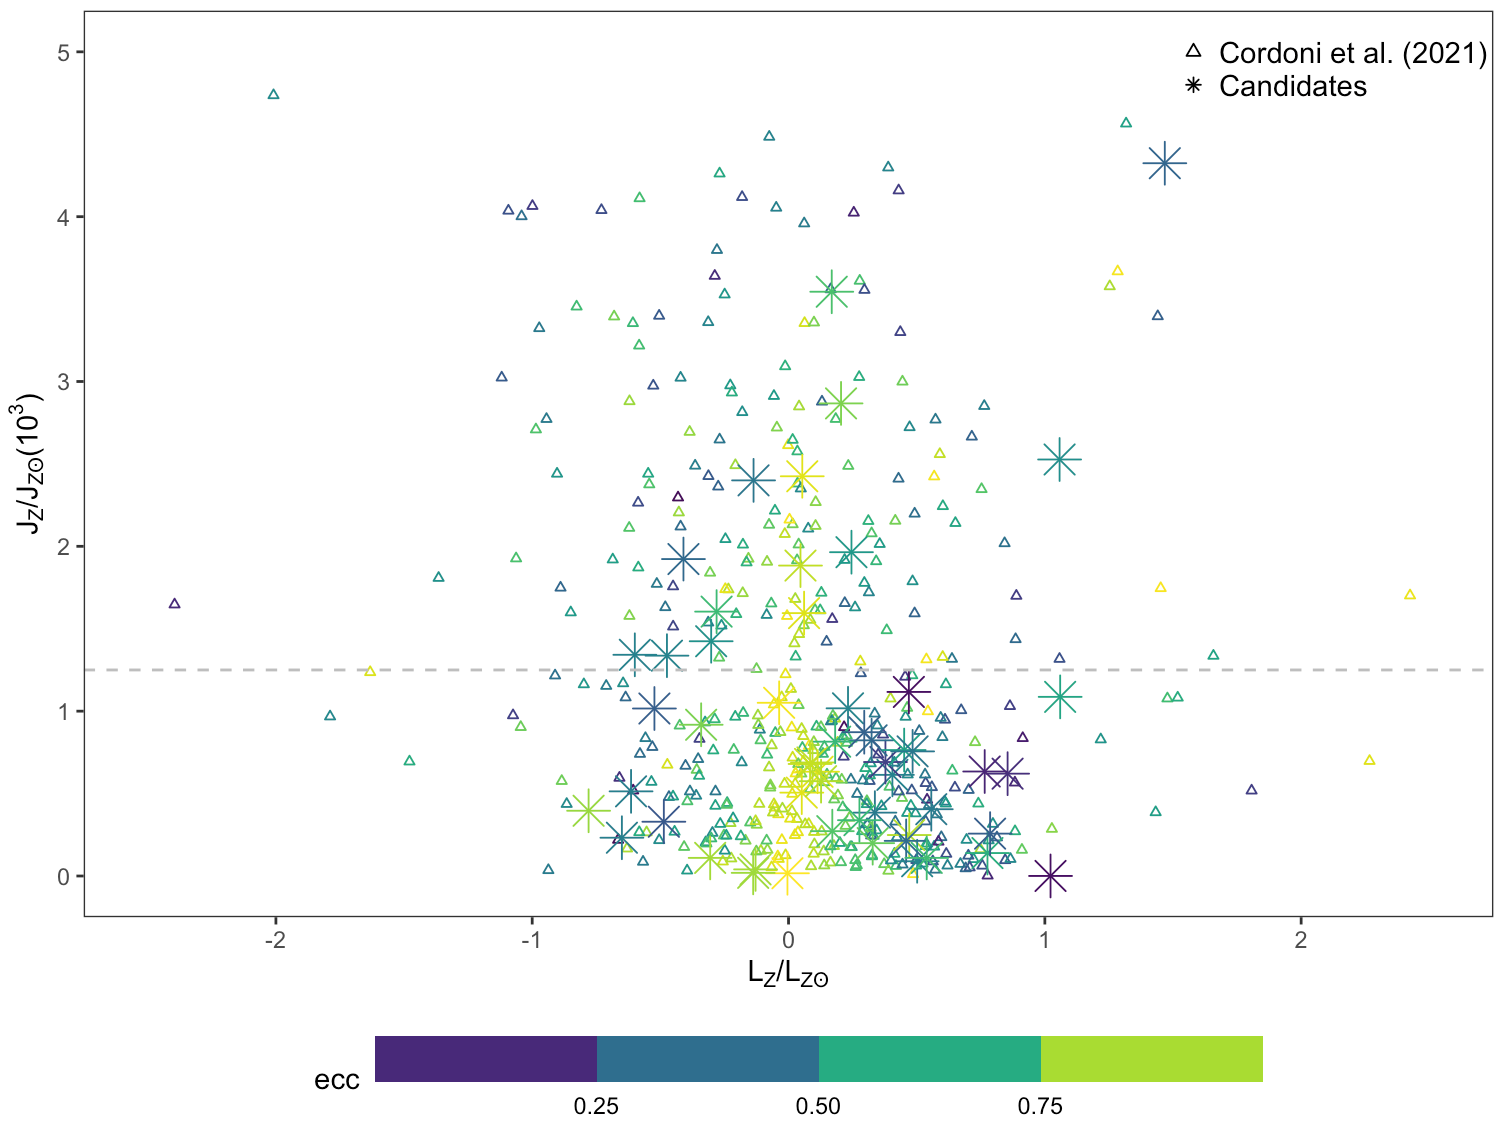
\includegraphics[width=\linewidth]{Plots/Figure14.png}
\caption{Vertical versus azimuthal action components color-coded by eccentricity for our EMP candidates with metallicities \feh $<-3$ (star symbol), as well as literature values from \citet[][triangle symbol]{Cordoni2021}. The action quantities are scaled by the solar values
(i.e.,  $L_{z \odot}=2009.92$ km s$^{−1}$ kpc, $J_{z \odot} =0.35$ km s$^{−1}$ kpc). In this parameter space, we adopt the same horizontal dashed line at $ \nicefrac {J_{z}}{J_{z \odot}} =1.25 \times 10^{3}$ as in \citet{Cordoni2021} to distinguish between planar and non-planar orbits. The distribution of our candidates appears to be consistent with the observed orbital properties of confirmed EMP stars shown in Figure 1 of \citet{Sestito2020} and Figure 5 of \citet{Cordoni2021}.}
\label{fig:candidate_orbitals}
\end{figure}

The orbital information for our EMP candidates is captured in the vertical action and azimuthal action plot shown in Figure~\ref{fig:candidate_orbitals}, similar to Figure 1 of \citet{Sestito2020} and Figure 5 of \citet{Cordoni2021}. While our admittedly smaller set of candidates does not extend as high in vertical action as the \citet{Sestito2020} sample, we do see a significant near-``planar'' component, biased toward prograde motion, in agreement with the results of both those authors and the Skymapper-based study of \citet{Cordoni2021}. Hence, while these kinematic data are not proof of the EMP nature of our candidates, they are consistent with the observed properties of confirmed EMP stars. 

Finally, we note that the method presented here evolved from \citet{hughes2017}, which employed \ts\ on GALAH spectra to classify them and identify several interesting classes of objects, including metal-poor stars. In that work the fit used a relatively simple set of absorption features in the spectra. In the present work, we found a significant improvement in the quality of the candidates by assessing different line combinations in order to improve our metallicity sensitivity (see Appendix~\ref{deriving lines}). We furthermore included the GALAH infrared fourth channel because it contains an oxygen feature -- not previously considered -- which served as a discriminant to reject spurious hot stars.


\subsection{Advantages of a machine learning-based approach over more traditional \texorpdfstring{\ci}\ fitting methods } \label{Sec:Method Comparison}

As shown in Figure~\ref{fig:tsne_map_zoomed}, our method uses \ts\ to isolate candidate \emps in a region with spectra similar to known \emps from the literature. By fitting synthetic spectra to the candidate \emps, we refine the selection of EMP candidates in the \ts\ space of EMP candidates to the top portion of the data shown in Figure~\ref{fig:estimate_elephants}. The clustering of known and candidate \emps in essentially a localised region in the entire \ts parameter space illustrates the potential power of our method. Nevertheless, a valid question is whether there are any improvements on our machine learning-based method in terms of finding \emps over a simple \ci \ fit to a wide range of synthetic spectral templates.

We tested the \ci stellar parameter routine on the full GALAH dataset, to potentially identify \emps \ that did not fall within the \ts EMP island identified in Figure~\ref{fig:tsne_map_zoomed}. The results of this run are compared to the \ts run in Table~\ref{tab:Candidate Counts}. The purely \ci method returned more potential candidates, but upon visual inspection,  81\%  of those candidates were poorly fit, and some had strong absorption features, indicating that they are not good EMP candidates. The increased fraction of bad fits is likely because of model systematics -- the minimum \ci \ might not be representative of actual EMPs. Applying \ts before running a \ci fitting routine minimises this effect.

Moreover, we found that the \ci method does not contain all the \ts~EMP candidate sample: only 10 of our total sample of 60 (54 candidates and 6 spurious stars)
are found. Finally we also note that not all of the literature stars from Table~\ref{tab:Metal-Poor_Table} were recovered in the \ci sample: only 3 of 23 are found.

\begin{table}
    \begin{tabular}{@{}lrrrl@{}}
    \hline
   Method   & \ \emps \ (\%) & Extraneous sources (\%) & Total EMP Candidates \\
    \hline
    \hline
    \ci \ only  &  19 & 81  & 126  \\
    \ts \ and \ci & 90 & 10  &  60
    \end{tabular}
    \caption{Accuracy percentages between our method (i.e. \ts\ classification, then a \ci \ fit to models) and a traditional \ci-fitting technique for finding \emps. Percentage of EMP stars is the fraction of the total count that passed a visual inspection. Extraneous sources included both candidates with bad fits and those with strong absorption features, indicating that they are not likely to be \emps. The accuracy percentage of candidates that were found to be good EMP stellar candidates is higher using our method.}
    \label{tab:Candidate Counts}
\end{table}

\section{Conclusions}\label{Sec:Conclusions}

We have demonstrated a methodology for finding \emps \ within a spectroscopic dataset -- in this case spectra of $\sim 600,000$ stars from the \g high-resolution survey -- that is both computationally efficient and accurate, and may potentially be adapted to find other specific types of stars. Furthermore we have shown that, using the \g \ wavelength ranges, we can derive metallicities down to \feh $\sim  -3.5$. 

The candidate list we have identified is distinct from the results of many past surveys targeted specifically at \emps \citep[e.g.,][]{Da_Costa_2019,Starkenburg2017}. Given the nature of the \g dataset -- essentially a magnitude-limited sample of stellar spectra -- our candidate list does not preferentially select giant stars (although, given their greater luminosity, giant stars probe a larger volume). This means we are sensitive to main-sequence and main-sequence turnoff stars, which are an interesting EMP population because, not having undergone dredge-ups, they are more likely to retain their original abundance patterns, and in the case of main-sequence turnoff stars, they can potentially yield useful stellar ages. Moreover the lack of strong carbon features in the \g wavelength windows means we are not biased against carbon-enhanced metal-poor stars -- a significant fraction of \emps \citep{Yong2013,2013AJ....146..132L} -- unlike some photometric-based \emp surveys \citep[cf.][]{Da_Costa_2019}.

With regard to our methodology, we found hybrid approach, i.e., pre-selection using \ts focused on specific wavelength regions, followed by parameter estimation via \ci-fitting, to be the most efficient way to identify candidate \emps. Simpler ``brute-force'' methods, for example applying \ts to the entire spectral range, or skipping machine-learning-based pre-selection and going straight to \ci-fitting to template spectra, proved to be both much more computationally intensive and much more likely to include extraneous spectra in their output. Although our method was tailored to \g spectra, we expect that similar techniques should be applicable to datasets from other ongoing and future large spectroscopic surveys, including WEAVE \citep{Dalton_2014} and 4MOST \citep{Jong20194MOSTPO}. 

While we have demonstrated that our metallicity estimates -- along with those from the \g DR3 pipeline -- are fairly reliable with regard to identifying \emp candidates, follow-up observations, ideally covering additional regions of the optical spectrum more sensitive to low-metallicity measurements, are required to confirm these estimates, as well as to determine the abundances of carbon and other specific elements of interest \citep[see, e.g.,][]{Beers2005, Frebel2015}. To this end we are engaged in a program of follow-up spectroscopy, with initial results expected shortly (Da Costa et al., in prep.).


\begin{acknowledgments}

We are grateful to the anonymous referee for their helpful comments and suggestions.
Parts of this research were supported by the Australian Research Council Centre of Excellence for All Sky Astrophysics in 3 Dimensions (ASTRO 3D), through project number CE170100013.  LS acknowledges support from  Australian Research Council Discovery Project DP190102448. DBZ, JS and SLM acknowledge support from Australian Research Council Discovery Project DP180101791. YST acknowledges support from the Australian Research Council through DECRA Fellowship DE220101520. This work was based on data acquired at the Anglo-Australian Telescope. We acknowledge the traditional custodians of the land on which the AAT stands, the Gamilaraay people, and pay our respects to elders past and present.

\vspace{5mm}
\facility{AAT:HERMES}

\software{Astropy \citep{astropy:2013, astropy:2018} \ Matplotlib \citep[][\url{http://dx.doi.org/10.1109/MCSE.2007.55}]{4160265} \ Rtsne \citep[][\url{https://github.com/jkrijthe/Rtsne}]{Rtsne}}

\end{acknowledgments}

% The best way to enter references is 
\bibliographystyle{mnras}
\bibliography{references} % if your bibtex file is called example.bib


% Alternatively you could enter them by hand, like this:
% This method is tedious and prone to error if you have lots of references
%\begin{thebibliography}{99}
%\bibitem[\protect\citeauthoryear{Author}{2012}]{Author2012}
%Author A.~N., 2013, Journal of Improbable Astronomy, 1, 1
%\bibitem[\protect\citeauthoryear{Others}{2013}]{Others2013}
%Others S., 2012, Journal of Interesting Stuff, 17, 198
%\end{thebibliography}

%%%%%%%%%%%%%%%%%%%%%%%%%%%%%%%%%%%%%%%%%%%%%%%%%%
%%%%%%%%%%%%%%%%% APPENDICES %%%%%%%%%%%%%%%%%%%%%
\appendix
\section{Deriving metallicities for metal-poor candidates with GALAH spectra}\label{deriving lines}

This Section describes a set of simulation outputs that illustrate (1) the sensitivity of using only GALAH spectra to estimate metallicity at low metallicities (\feh $\sim-4.5$ is possible for cool giants) and (2) refine the line list we use for the low metallicity fits (the three bluer channels are preferred slightly over a few strong Fe lines).

The simulations work by adding realistic noise to synthetic stellar templates with known parameters, and attempting to recover \feh \ using the same templates.  We fix [$\alpha$/H]$=0.4$ and consider a limited range of Carbon enhancements ([C/H]$=0.0, 0.5, 1.0$). 

It is important to note that the following simulation results are only for fitting \feh. We assume that \logg \ and \teff \ are already well-constrained (see Section~\ref{sec:galah} for how we do this with GALAH spectra) so we can limit the number of templates we fit to. The simulation results below did consider different carbon enhancements, in the sense that we explored whether carbon enhancement impacts the metallicity sensitivities. This means the current simulations were not meant to test our ability to constrain Carbon abundance in an individual spectrum.

As shown in Section~\ref{Sec:Results}, the current sample of candidate \emps have a median S/N of $35$ and two rough sub-populations: cool giants (\teff $=5000$, \logg $\sim 2$) and hot main sequence stars (\teff $=6000$, \logg $ \sim 4$).

To find the best regions of the GALAH spectra to fit for metallicity, we considered two different line lists as well as fitting to entire HERMES spectral channels. The first line list is from T. Nordlander and is highlighted shown in Figure~\ref{fig:thomas_synthetic}. The second is a list of 57 metal-sensitive (mostly iron) lines compiled from features found in synthetic spectra and observed stars around \feh$\sim-3$ from K. Venn (priv. comm.).

\begin{figure}
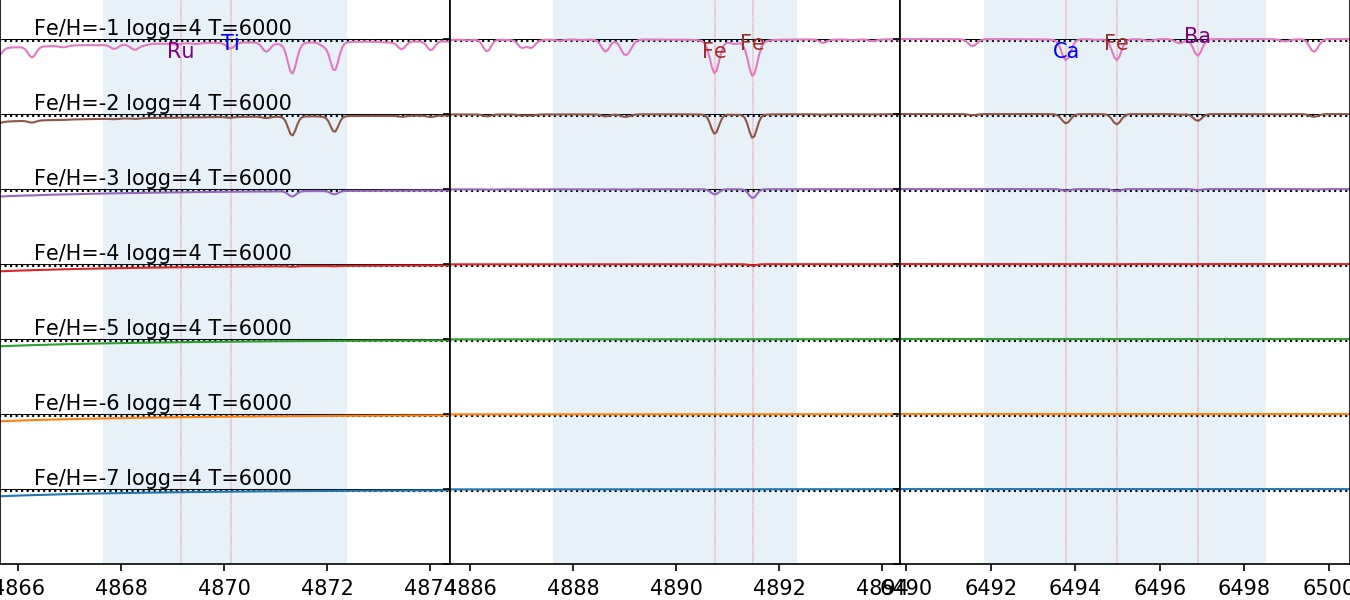
\includegraphics[width=\linewidth]{Plots/sim_plots/plot_thomas_regions_synthetic.jpg}
\caption{A plot of synthetic spectra of a hot main sequence star for a range of metallicities. The blue shaded areas are the wavelength regions with metal-sensitive absorption features.}
\label{fig:thomas_synthetic}
\end{figure}

Figure~\ref{fig:simulation} shows the output from one run of the simulation on the strongest features. Parameters for the input spectra are given in the title and the number of simulated stars for each input \feh was set to N$_{sims}=10000$. The results show that for this spectral line that metallicity is well-constrained until \feh $\sim-4.5$. For lower metallicities the simulation indicates S/N=35 spectral data over this line cannot distinguish between \feh $\sim-5$ to $-7$ values.

\begin{figure}
    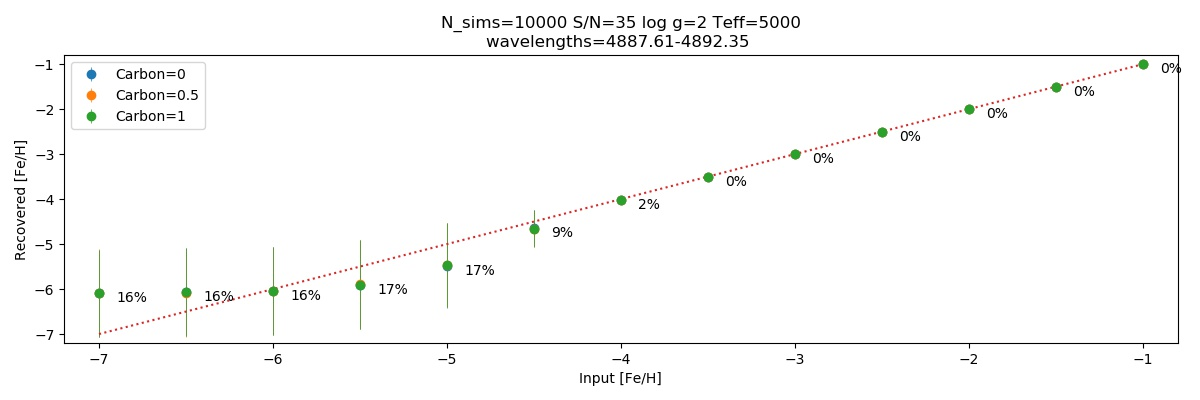
\includegraphics[width=\linewidth]{Plots/sim_plots/Nsim10000_SN35_logg2_T5000_Thomas_4890.jpg}
    \caption{Simulation results for recovering input metallicities of synthetic cool giant stellar spectra, with noise typical of the current sample. The points represent the recovered mean \feh with error bars reflecting the standard deviation in individual recovered \feh values. Percentages are the fractional uncertainty on the recovered metallicity. 
    The data suggest we can constrain metallicity to within $\sim8\%$ down to \feh $\sim-4.5$ for cool giants and data with S/N$=35$. For lower input metallicities, the simulation results indicate the spectra have essentially no constraint on metallicities \feh $<-4.5$ at S/N$=35$. The carbon abundances of the input spectra do not appear to impact the metallicity sensitivity as can be seen by the carbon abundance of 1 (green) overlaying both the carbon abundance of 0 and 0.5 ( blue and orange respectively).}
    \label{fig:simulation}
\end{figure}

Figure~\ref{fig:multiple_lines} shows simulation runs where multiple spectral lines were simultaneously fit to illustrate improvement in metallicity constraints. While the second strongest set of lines improves the fitting to lower metallicities, the third set of lines does not influence the measured metallicity significantly for S/N=35 spectra.

\begin{figure}
\subfloat[]{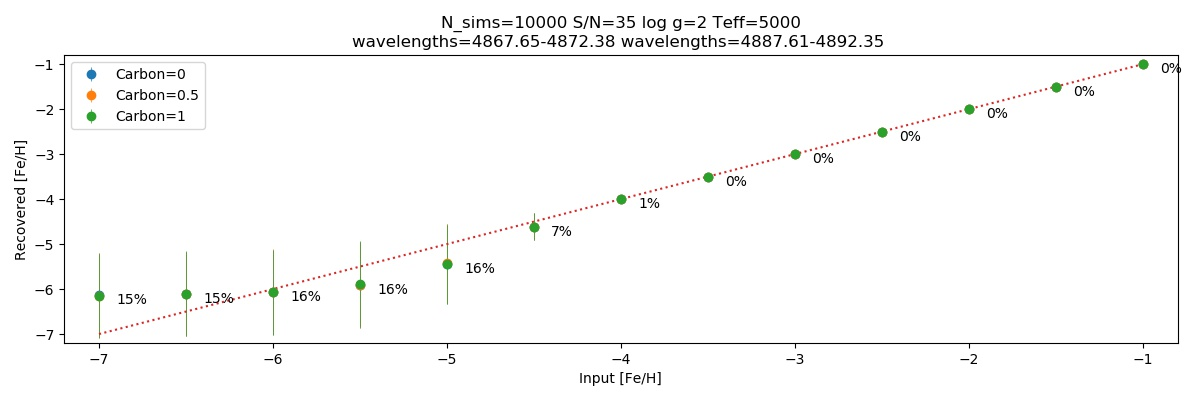
\includegraphics[width=\linewidth]{Plots/sim_plots/Nsim10000_SN35_logg2_T5000_Thomas_4870_4890.jpg}}

\subfloat[]{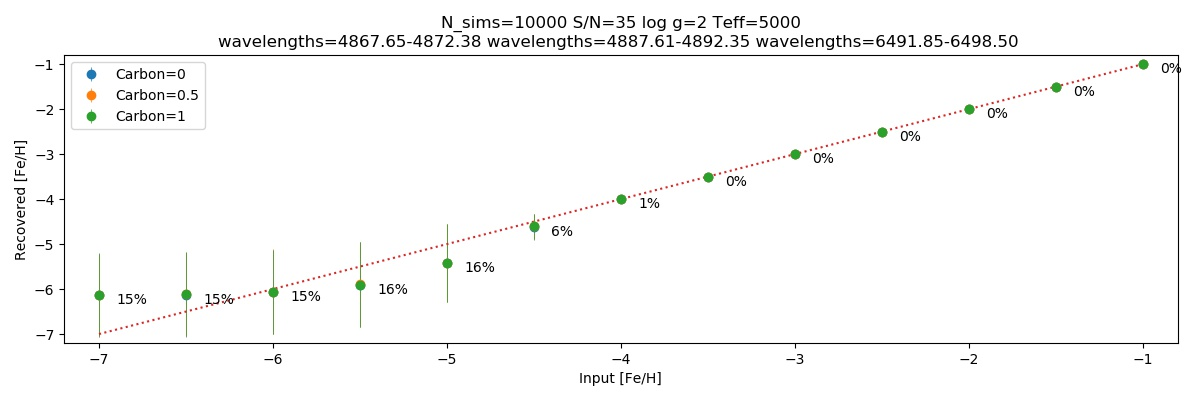
\includegraphics[width=\linewidth]{Plots/sim_plots/Nsim10000_SN35_logg2_T5000_Thomas_4870_4890_6495.jpg}}

\caption{Same format as Figure~\ref{fig:simulation}, now with panels showing two different combinations of spectral lines shown in Figure~\ref{fig:thomas_synthetic}, as indicated in the panel's subtitle. While the joint constraint of the spectral regions with the strongest features yields a better \feh~constraint compared to a single line ($cf.$ Figure~\ref{fig:simulation}), the third spectral region does not improve the fits for this stellar type and assumed S/N, likely because its features are weaker.}
\label{fig:multiple_lines}
\end{figure}

Figure~\ref{fig:final_cool_giant} shows metallicity sensitivity simulations for an additional line lists (K. Venn, priv. comm.) with 57 features as well as full fits to the spectra over the 3 HERMES channels. These are compared to the best combination of 2 lines from Figure~\ref{fig:multiple_lines}. Increased wavelength coverage appears to yield better metallicity constraints in the simulations, but only marginally so. 

\begin{comment}
\subfloat[]{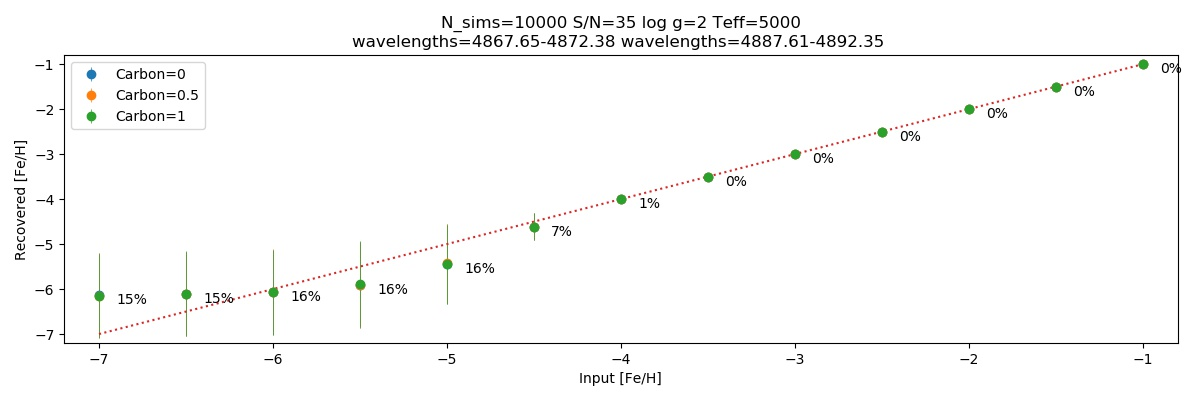
\includegraphics[width=\linewidth]{Plots/sim_plots/Nsim10000_SN35_logg2_T5000_Thomas_4870_4890.jpg}}

\subfloat[]{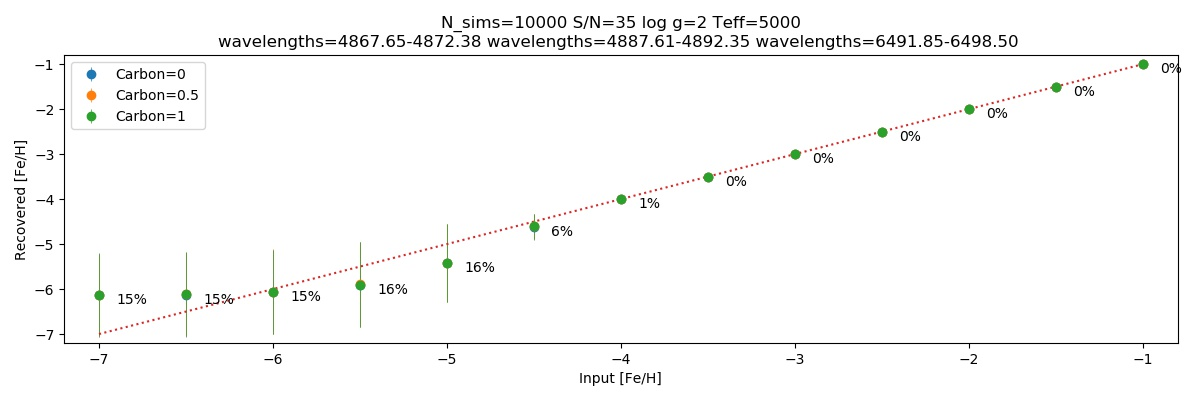
\includegraphics[width=\linewidth]{Plots/sim_plots/Nsim10000_SN35_logg2_T5000_Thomas_4870_4890_6495.jpg}}

\caption{Same format as Figure~\ref{fig:simulation}, now with panels showing two different combinations of spectral lines shown in Figure~\ref{fig:thomas_synthetic} as indicated in the panel's subtitle. While the joint constraint of the spectral regions with the strongest features yields a better \feh constraint compared to a single line (c.f. Figure~\ref{fig:simulation}), the third spectra region does not improve the fits for this stellar type and assumed S/N likely because its features are weaker.
}
\label{fig:alternative_line_lists}
\end{comment}


\begin{figure}
\subfloat[]{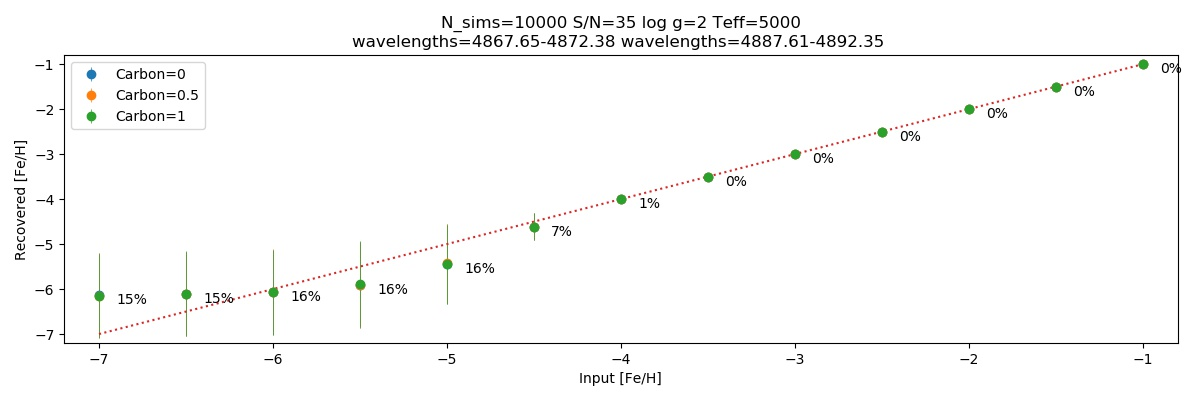
\includegraphics[width=\linewidth]{Plots/sim_plots/Nsim10000_SN35_logg2_T5000_Thomas_4870_4890.jpg}}

\subfloat[]{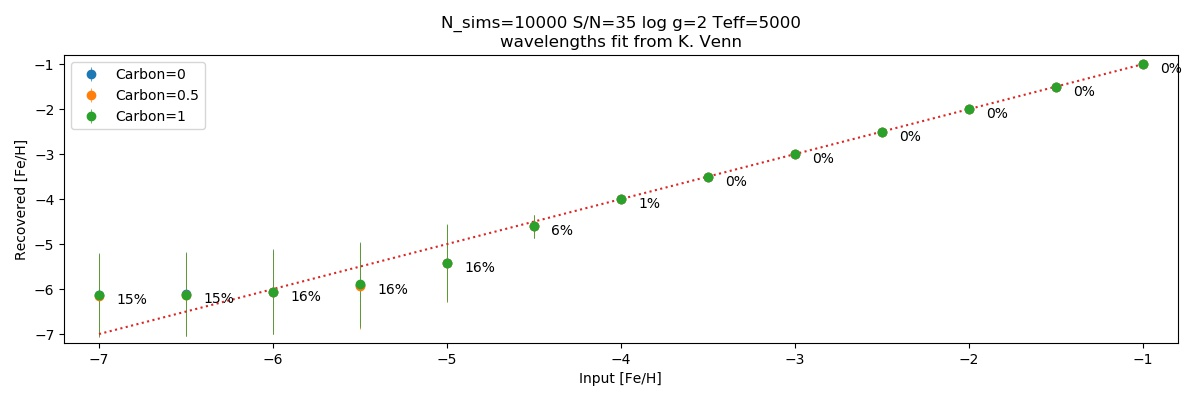
\includegraphics[width=\linewidth]{Plots/sim_plots/Nsim10000_SN35_logg2_T5000_All_Kim_Lines.jpg}}

\subfloat[]{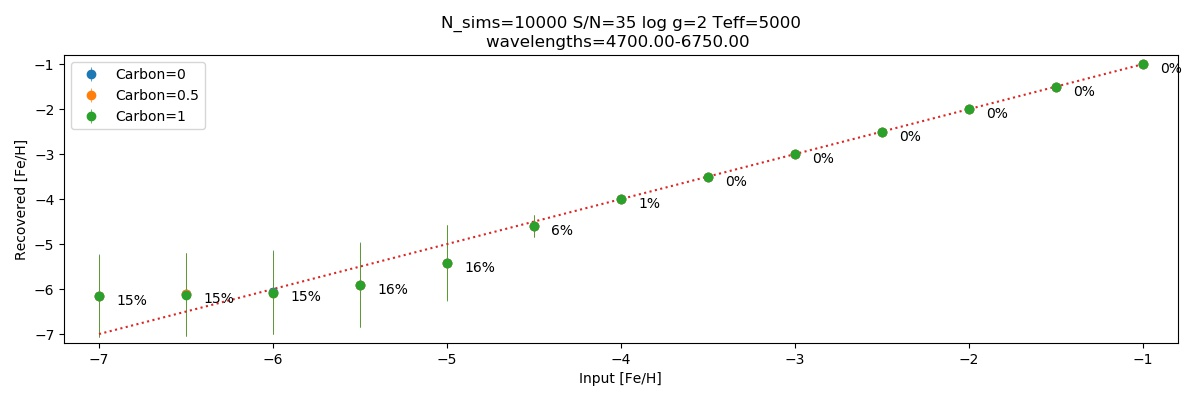
\includegraphics[width=\linewidth]{Plots/sim_plots/Nsim10000_SN35_logg2_T5000_GALAH_Channels_1-3.jpg}}

\caption{Same format as Figure~\ref{fig:simulation}, now with panels showing three different combinations of spectral lines: top is the Nordlander best features (Figure~\ref{fig:multiple_lines}), middle is fit to 57 metal-sensitive features (K. Venn, priv. comm) and the bottom plot shows fitting results to the first 3 HERMES Channels. The fit to 3 spectral channels yields a marginally better constraint at \feh $\sim-4.5$ for cool giants with S/N=35 than fits for \feh to the other spectra regions.
}
\label{fig:final_cool_giant}
\end{figure}

We show simulation results for hot main sequence stars in Figure~\ref{fig:final_hot_main_sequence}. At these temperatures, the metallicity sensitivity decreases, so that only metallicities of \feh $\sim-3.5$ or higher are measurable with S/N=35 GALAH spectra.

\begin{figure}
\subfloat[]{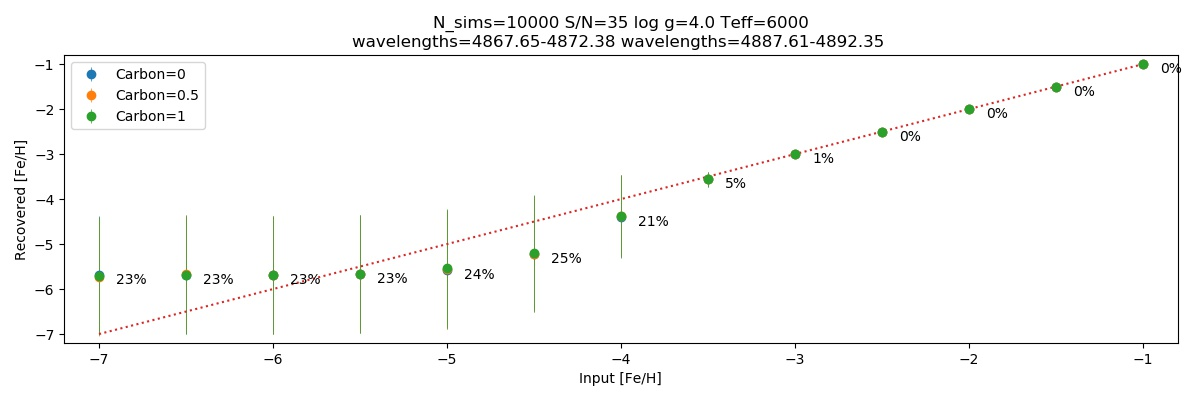
\includegraphics[width=\linewidth]{Plots/sim_plots/Nsim10000_SN35_logg4.0_T6000_Thomas_4870_4890.jpg}}

\subfloat[]{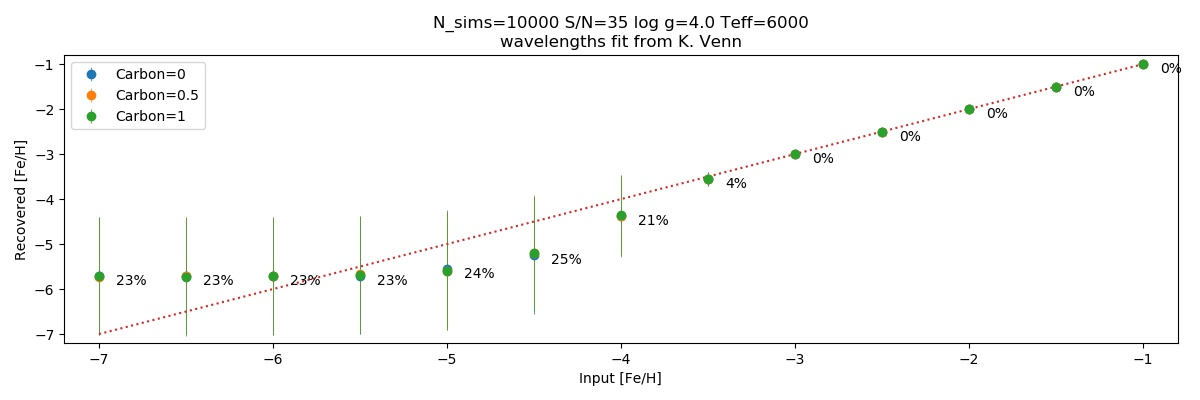
\includegraphics[width=\linewidth]{Plots/sim_plots/Nsim10000_SN35_logg4.0_T6000_All_Kim_Lines.jpg}}

\subfloat[]{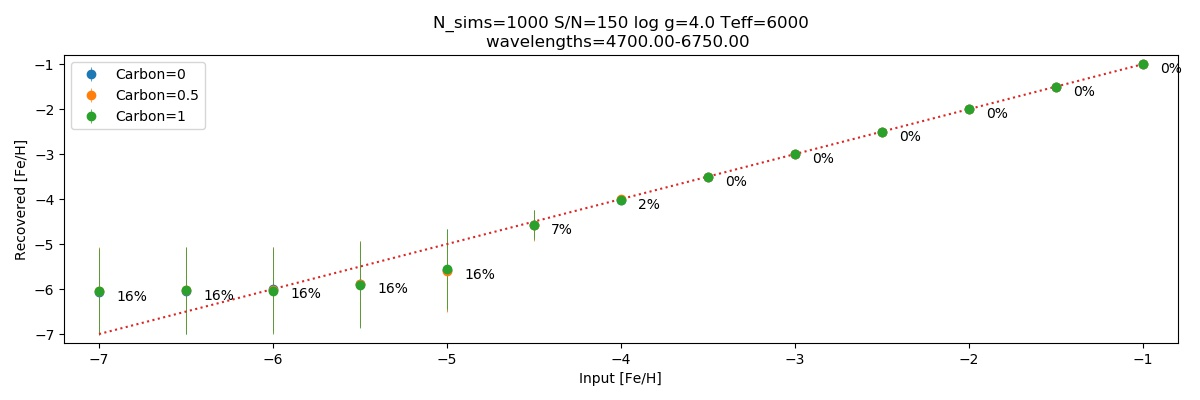
\includegraphics[width=\linewidth]{Plots/sim_plots/Nsim1000_SN150_logg4.0_T6000_GALAH_Channels_1-3.jpg}}
 
\caption{Same as Figure~\ref{fig:final_cool_giant} now for hot (\teff $=6000$) main sequence (\logg $=4$) stellar templates. Overall the metallicity sensitivity decreases such that we may only expect to make measurements to \feh $\sim-3.5$.
}
\label{fig:final_hot_main_sequence}
\end{figure}


Finally, we show in Figure~\ref{fig:high_sn_sim} how the metallicity sensitivity is expected to improve for higher S/N (S/N $\sim 150$) data: \feh $\sim-5.0$ and $\sim-4$ are expected for cool giants and hot main sequence stars, respectively.

\begin{figure}
\subfloat[]{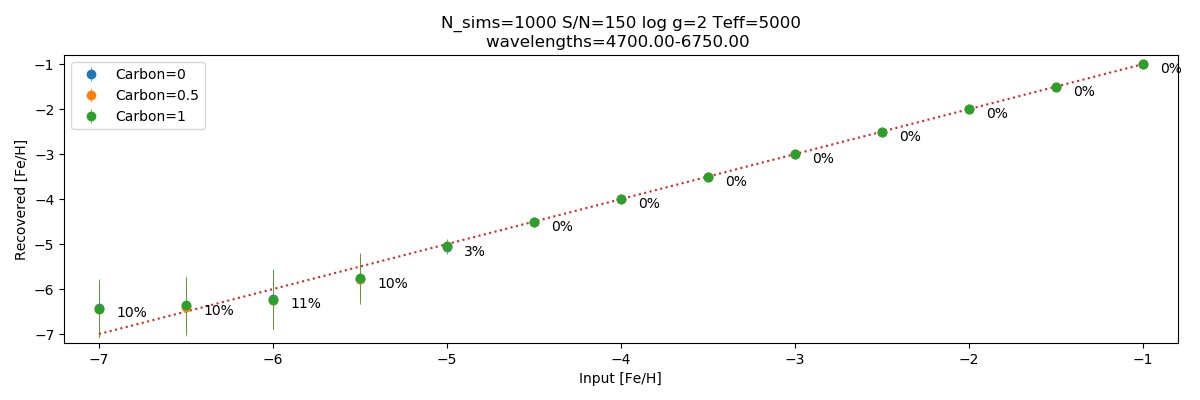
\includegraphics[width=\linewidth]{Plots/sim_plots/Nsim1000_SN150_logg2_T5000_GALAH_Channels_1-3.jpg}}

\subfloat[]{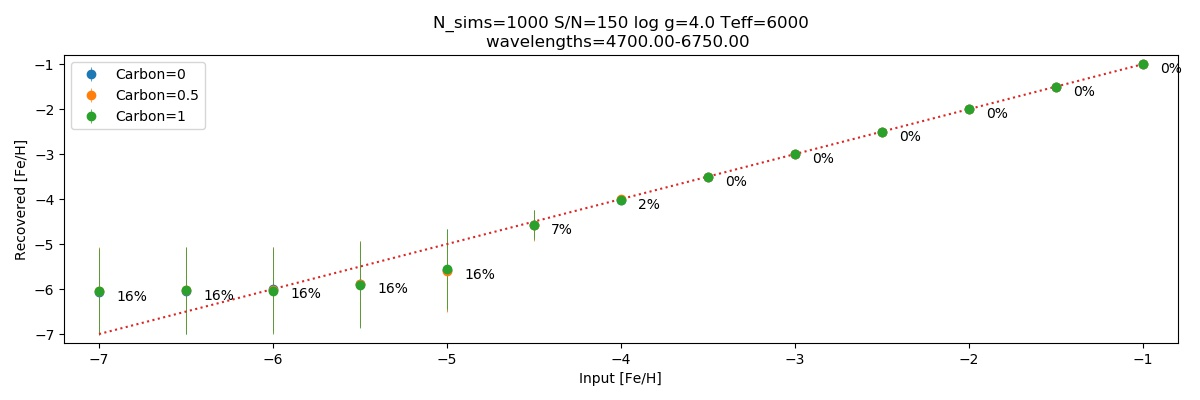
\includegraphics[width=\linewidth]{Plots/sim_plots/Nsim1000_SN150_logg4.0_T6000_GALAH_Channels_1-3.jpg}}


\caption{A few spectra in the GALAH sample reach S/N=150. These simulations show how much better the low metallicity constraints can be with higher S/N data and fits over the entire first 3 GALAH Channels.
}
\label{fig:high_sn_sim}
\end{figure}

To conclude, we find:
\begin{itemize}
    \item Synthetic cool giant spectra with typical GALAH S/N$=35$ over the GALAH spectral range are good ($\sim9\%$) at recovering metallicities as low as \feh $\sim-5.5$. 
    \item At a certain metallicity the GALAH spectra are no longer sensitive to lower metallicities for S/N=35 spectra.
    \item With better S/N($\sim 100$, or even $\sim 150$), metallicities as low as \feh $\sim-4.5$ can be recovered to $\sim9\%$.
    \item The metallicity sensitivity and fitting does not appear to be impacted by the level of carbon enhancement of the star within the wavelength coverage of the GALAH spectral channels.
\end{itemize}

\end{document}

% End of file `sample631.tex'.
